\def\year{2022}\relax
%File: formatting-instructions-latex-2022.tex
%release 2022.1
\documentclass[letterpaper]{article} % DO NOT CHANGE THIS
\usepackage{aaai22}  % DO NOT CHANGE THIS
\usepackage{times}  % DO NOT CHANGE THIS
\usepackage{helvet}  % DO NOT CHANGE THIS
\usepackage{courier}  % DO NOT CHANGE THIS
\usepackage[hyphens]{url}  % DO NOT CHANGE THIS
\usepackage{graphicx} % DO NOT CHANGE THIS
\urlstyle{rm} % DO NOT CHANGE THIS
\def\UrlFont{\rm}  % DO NOT CHANGE THIS
\usepackage{natbib}  % DO NOT CHANGE THIS AND DO NOT ADD ANY OPTIONS TO IT
\usepackage{caption} % DO NOT CHANGE THIS AND DO NOT ADD ANY OPTIONS TO IT
\DeclareCaptionStyle{ruled}{labelfont=normalfont,labelsep=colon,strut=off} % DO NOT CHANGE THIS
\frenchspacing  % DO NOT CHANGE THIS
\setlength{\pdfpagewidth}{8.5in}  % DO NOT CHANGE THIS
\setlength{\pdfpageheight}{11in}  % DO NOT CHANGE THIS

%
% These are recommended to typeset algorithms but not required. See the subsubsection on algorithms. Remove them if you don't have algorithms in your paper.
\usepackage{algorithm}
\usepackage{algorithmic}
\usepackage{comment}
\usepackage{xcolor}
\usepackage{amsmath}
\usepackage{amssymb}
\usepackage{amsfonts}
\usepackage{subfig}
\usepackage{makecell}
\usepackage{arydshln}

\newcommand{\std}[1]{\fontsize{9}{10}\selectfont \emph{(#1)} \fontsize{10}{10}\selectfont}
\newcommand{\junwen}[1]{\textcolor{blue}{ #1 (Junwen)}}
\newcommand{\joshua}[1]{\textcolor{purple}{ #1 (Joshua)}}

\newcommand{\carla}[1]{\textcolor{magenta}{ #1}}
%
% These are are recommended to typeset listings but not required. See the subsubsection on listing. Remove this block if you don't have listings in your paper.
\usepackage{newfloat}
\usepackage{listings}
\lstset{%
	basicstyle={\footnotesize\ttfamily},% footnotesize acceptable for monospace
	numbers=left,numberstyle=\footnotesize,xleftmargin=2em,% show line numbers, remove this entire line if you don't want the numbers.
	aboveskip=0pt,belowskip=0pt,%
	showstringspaces=false,tabsize=2,breaklines=true}
\floatstyle{ruled}
\newfloat{listing}{tb}{lst}{}
\floatname{listing}{Listing}
%
%\nocopyright
%
% PDF Info Is REQUIRED.
% For /Title, write your title in Mixed Case.
% Don't use accents or commands. Retain the parentheses.
% For /Author, add all authors within the parentheses,
% separated by commas. No accents, special characters
% or commands are allowed.
% Keep the /TemplateVersion tag as is
\pdfinfo{
/Title (AAAI Press Formatting Instructions for Authors Using LaTeX -- A Guide)
/Author (AAAI Press Staff, Pater Patel Schneider, Sunil Issar, J. Scott Penberthy, George Ferguson, Hans Guesgen, Francisco Cruz, Marc Pujol-Gonzalez)
/TemplateVersion (2022.1)
}

% DISALLOWED PACKAGES
% \usepackage{authblk} -- This package is specifically forbidden
% \usepackage{balance} -- This package is specifically forbidden
% \usepackage{color (if used in text)
% \usepackage{CJK} -- This package is specifically forbidden
% \usepackage{float} -- This package is specifically forbidden
% \usepackage{flushend} -- This package is specifically forbidden
% \usepackage{fontenc} -- This package is specifically forbidden
% \usepackage{fullpage} -- This package is specifically forbidden
% \usepackage{geometry} -- This package is specifically forbidden
% \usepackage{grffile} -- This package is specifically forbidden
% \usepackage{hyperref} -- This package is specifically forbidden
% \usepackage{navigator} -- This package is specifically forbidden
% (or any other package that embeds links such as navigator or hyperref)
% \indentfirst} -- This package is specifically forbidden
% \layout} -- This package is specifically forbidden
% \multicol} -- This package is specifically forbidden
% \nameref} -- This package is specifically forbidden
% \usepackage{savetrees} -- This package is specifically forbidden
% \usepackage{setspace} -- This package is specifically forbidden
% \usepackage{stfloats} -- This package is specifically forbidden
% \usepackage{tabu} -- This package is specifically forbidden
% \usepackage{titlesec} -- This package is specifically forbidden
% \usepackage{tocbibind} -- This package is specifically forbidden
% \usepackage{ulem} -- This package is specifically forbidden
% \usepackage{wrapfig} -- This package is specifically forbidden
% DISALLOWED COMMANDS
% \nocopyright -- Your paper will not be published if you use this command
% \addtolength -- This command may not be used
% \balance -- This command may not be used
% \baselinestretch -- Your paper will not be published if you use this command
% \clearpage -- No page breaks of any kind may be used for the final version of your paper
% \columnsep -- This command may not be used
% \newpage -- No page breaks of any kind may be used for the final version of your paper
% \pagebreak -- No page breaks of any kind may be used for the final version of your paper
% \pagestyle -- This command may not be used
% \tiny -- This is not an acceptable font size.
% \vspace{- -- No negative value may be used in proximity of a caption, figure, table, section, subsection, subsubsection, or reference
% \vskip{- -- No negative value may be used to alter spacing above or below a caption, figure, table, section, subsection, subsubsection, or reference

\setcounter{secnumdepth}{0} %May be changed to 1 or 2 if section numbers are desired.

% The file aaai22.sty is the style file for AAAI Press
% proceedings, working notes, and technical reports.
%

% Title

% Your title must be in mixed case, not sentence case.
% That means all verbs (including short verbs like be, is, using,and go),
% nouns, adverbs, adjectives should be capitalized, including both words in hyphenated terms, while
% articles, conjunctions, and prepositions are lower case unless they
% directly follow a colon or long dash
\title{A GNN-RNN Approach for Harnessing Geospatial and Temporal Information:\\  Application to  Crop Yield Prediction}
% \title{\carla{A GNN-RNN Approach for Harnessing Geospatial and Temporal Information:\\  Application to  Crop Yield Prediction}}



% \author{%
%   Joshua Fan\thanks{Equal contribution.} \\
%   Computer Science\\
%   Cornell University\\
%   Ithaca, NY 14853 \\
%   \texttt{jyf6@cornell.edu}
%   % examples of more authors
%   \And
%   Junwen Bai\footnotemark[1] \\
%   Computer Science \\
%   Cornell University \\
%   Ithaca, NY 14853 \\
%   \texttt{jb2467@cornell.edu} \\
%   \And
%   Zhiyun Li\footnotemark[1] \\
%   Applied Economics and Management \\
%   Cornell University \\
%   Ithaca, NY 14853 \\
%   \texttt{zl547@cornell.edu}
%   \And
%   Ariel Ortiz-Bobea \\
%   Applied Economics and Management \\
%   Cornell University \\
%   Ithaca, NY 14853 \\
%   \texttt{ao332@cornell.edu} 
%   \And
%   Carla Gomes \\
%   Computer Science \\
%   Cornell University \\
%   Ithaca, NY 14853 \\
%   \texttt{gomes@cs.cornell.edu}
% }


%Example, Single Author, ->> remove \iffalse,\fi and place them surrounding AAAI title to use it
\iffalse
\title{My Publication Title --- Single Author}
\author {
    Author Name
}
\affiliations{
    Affiliation\\
    Affiliation Line 2\\
    name@example.com
}
\fi

%\iffalse
% %Example, Multiple Authors, ->> remove \iffalse,\fi and place them surrounding AAAI title to use it
% \title{My Publication Title --- Multiple Authors}
% \author {
%     % Authors
%     First Author Name,\textsuperscript{\rm 1}
%     Second Author Name, \textsuperscript{\rm 2}
%     Third Author Name \textsuperscript{\rm 1}
% }
% \affiliations {
%     % Affiliations
%     \textsuperscript{\rm 1} Affiliation 1\\
%     \textsuperscript{\rm 2} Affiliation 2\\
%     firstAuthor@affiliation1.com, secondAuthor@affilation2.com, thirdAuthor@affiliation1.com
% }

%\iffalse
\author{
    %Authors
    % All authors must be in the same font size and format.
    Joshua Fan\thanks{Equal contribution.}\textsuperscript{\rm 1}, Junwen Bai\footnotemark[1]\textsuperscript{\rm 1},  Zhiyun Li\footnotemark[1]\textsuperscript{\rm 2},  Ariel Ortiz-Bobea\textsuperscript{\rm 2}, Carla P. Gomes\textsuperscript{\rm 1}\\
}
\affiliations{
    %Afiliations
    \textsuperscript{\rm 1} Department of Computer Science, Cornell University, USA\\
    \textsuperscript{\rm 2} Department of Applied Economics \& Management, Cornell University, USA\\
    % If you have multiple authors and multiple affiliations
    % use superscripts in text and roman font to identify them.
    % For example,
    % Sunil Issar, \textsuperscript{\rm 2}
    % J. Scott Penberthy, \textsuperscript{\rm 3}
    % George Ferguson,\textsuperscript{\rm 4}
    % Hans Guesgen, \textsuperscript{\rm 5}.
    % Note that the comma should be placed BEFORE the superscript for optimum readability
    % 2275 East Bayshore Road, Suite 160\\
    % Palo Alto, California 94303\\
    % email address must be in roman text type, not monospace or sans serif
    \{jyf6, jb2467, zl547, ao332\}@cornell.edu, gomes@cs.cornell.edu
}
%\fi


% REMOVE THIS: bibentry
% This is only needed to show inline citations in the guidelines document. You should not need it and can safely delete it.
\usepackage{bibentry}
% END REMOVE bibentry


\begin{document}

\maketitle

\begin{abstract}
Climate change is posing new challenges to crop-related concerns, including food insecurity, supply stability, and economic planning. Accurately predicting crop yields is crucial for addressing these challenges. However, this prediction task is exceptionally complicated since crop yields depend on numerous factors such as weather, land surface, and soil quality, as well as their interactions. In recent years, machine learning models have been successfully applied in this domain. However, these models either restrict their tasks to a relatively small region, or only study over a single or few years, which makes them hard to generalize spatially and temporally. In this paper, we introduce a novel graph-based recurrent neural network for crop yield prediction, to incorporate both geographical and temporal knowledge in the model, and further boost predictive power. Our method is trained, validated, and tested on over 2000 counties from 41 states in the US mainland, covering years from 1981 to 2019. As far as we know, this is the first machine learning method that embeds geographical knowledge in crop yield prediction and predicts crop yields at the county level nationwide. We also laid a solid foundation by comparing our model on a nationwide scale with other well-known baseline methods, including linear models, tree-based models, and deep learning methods. Experiments show that our proposed method consistently outperforms the existing state-of-the-art methods on various metrics, validating the effectiveness of geospatial and temporal information. 

%Climate change is posing new challenges to crop-related concerns including food insecurity, supply stability and economic planning. As one of the central challenges, crop yield prediction has become a pressing task in the machine learning field. Despite its importance, the prediction task is exceptionally complicated since crop yields depend on various factors such as weather, land surface, soil quality as well as their interactions. In recent years, machine learning models have shown many successful applications in the crop domain. However, these models either restrict their tasks to a relatively small region, or only span over a single or few years, which makes them hard to generalize spatially and temporally. In this paper, we present a new crop yield dataset comprising of plenteous weather, land, soil variables across over 3000 counties from all 48 states in the US mainland, covering years from 1981 to 2019. As far as we know, this is the first nationwide dataset with such a long time span in the crop domain for machine learning. On this dataset, we lay a solid foundation for machine learning tasks by applying well-known linear models, tree-based models, deep learning methods and comparing their performance. Moreover, we introduce a novel graph-based recurrent neural network for crop yield prediction, to incorporate both geographical and temporal knowledge in the model, and further boost the predictive power.
\end{abstract}

\section{Introduction}
From cleaning robots to self-driving cars, autonomous and semi-autonomous agents are becoming increasingly prevalent~\cite{stone2016artificial}. People's understanding of such agents' behaviors can increase their trust in the agents and their ability to collaborate with them~\cite{devin2016implemented,glass2008toward}. An understanding of an agent's behavior could also support people in tasks such as choosing between alternative agents and determining when the agent can be trusted with performing a task autonomously and when the user's attention is needed. For example, if a user can anticipate the behavior of  a self-driving car in different scenarios, she could be more prepared to take control in situations where the car might not perform well on its own.

While prior work has suggested ways to explain individual decisions of an agent to a person~\cite{khan2009minimal,khan2011automatically}, these approaches do not convey a ``global'' view of an agent's policy. Similarly, recent methods for interpretable machine learning~\cite{vellido2012making,doshi2017towards} typically explain a single decision made by a model, e.g. by presenting a simplified model which justifies decisions in a certain region in the space~\cite{ribeiro2016model}. In this paper, we introduce the problem of providing users with a summary of an agent's behavior. This approach aims to provide users with an overview of the agent's global strategy rather than explaining specific decisions  after the fact. 

A trivial way of communicating an agent's behavior is to show past executions or simulations. This approach, however, has important drawbacks. First, many of the situations an agent encounters might be uninteresting to a person (e.g., a self-driving car stuck in traffic for an hour). Second, reviewing long execution traces will require a person to spend a significant amount of time, and people might give up early, or not pay attention, potentially missing important states. Therefore, we seek solutions that extract \emph{effective} summaries which show the actions taken by the agent in key scenarios. Such summaries can reduce the human effort required to review the agent's behavior, while still providing sufficient information about its capabilities. We note that this is analogous to the approach taken in many settings in which people need to assess the performance of other people. For example, sports scouting agencies typically prepare videos that include highlights from players' games to demonstrate their skills\footnote{e.g.,  \url{https://www.youtube.com/watch?v=gX3e0UM-OeM}. We note that while such scouting videos are often biased to showcase only successful actions, we intend that summaries of agent behavior will include states that demonstrates their behavior in different states of interest, whether successful or not.}.  

%The approach of generating summaries that highlight the capabilities of agents is analogous to other settings in which people need to review the performance of other people. For example, sports scouting agencies prepare videos that include highlights from players' games to demonstrate their skills.\footnote{e.g.,  \url{https://www.youtube.com/watch?v=gX3e0UM-OeM}.}

We developed ``HIGHLIGHTS'', an algorithm that extracts important states from an execution trace of an agent in an online manner. Intuitively, a state is important if different actions in that states can lead to substantially different outcomes for the agent. For example, deciding which turn to take when driving in a city will not be considered important if taking the next turn will result in a similar arrival time; deciding whether to exit a highway will be considered more important, as missing the exit can result in a significant delay. Our approach assumes that HIGHLIGHTS has access to the agent's strategy which is described using a  Markov Decision Process (MDP) policy, and quantifies the importance of states based on the agent's Q-values. To provide more context to the user, rather than showing important states in isolation, the algorithm extracts a trajectory that includes neighboring states and composes a summary of the agent's behavior from these trajectories.

We used HIGHLIGHTS to create summaries of agents playing Mrs. Pacman~\cite{rohlfshagen2011ms} and evaluated these summaries in a human-subject experiment. We compared HIGHLIGHTS summaries with two baselines. One baseline generated summaries by extracting random trajectories of the agent, which will, on average, include states that are more likely to be encountered. The other baseline generated summaries by extracting the first trajectories the agent encountered, which is akin to having a user watch the agent until she runs out of time. In the experiment, participants were shown summaries of different Pacman agents which varied in their performance, and were asked to select an agent to play on their behalf.  They were also asked to rate the helpfulness of different summaries for evaluating an agent's capabilities. 
%They were also shown pairs of summaries of the \emph{same} Pacman agent and were asked to subjectively assess how helpful each of the summaries is for understanding that agent's capabilities. 
Our results show that HIGHLIGHTS led to improved objective performance of participants: they were significantly more likely to choose the better performing agent when the HIGHLIGHTS summaries were shown. HIGHLIGHTS summaries were also rated as more helpful by the study participants. 

%can be condensed to two sentences if needed
One limitation of the HIGHLIGHTS algorithm is that it does not consider the diversity of states in the summary, and therefore if important states are similar to each other, the summary will consist of similar trajectories, thus conveying less new information to users. To mitigate this problem, we developed a variant of the HIGHLIGHTS algorithm which, in addition to state importance, takes into consideration the similarity of the state to other states in the summary. This extension further improved participants' ability to assess the performance of different agents.

The contributions of the paper are threefold: (1) we introduce and formalize the problem of summarizing an agent's behavior to people; (2) we develop HIGHLIGHTS and HIGHLIGHTS-DIV, algorithms that automatically extract summaries of an agent's policy, and (3) we conduct human-subject experiments, showing that summaries generated by HIGHLIGHTS and HIGHLIGHTS-DIV were preferred by participants and improved their ability to assess the capabilities of agents compared to the baseline summaries.


% \section{Task Formulation and Dataset}
\label{sec:datasets}
 
Fig. \ref{fig:neuronal-data} briefly illustrates the general pipeline of large-scale neuron reconstruction from EM image volume and various data used in our work.
The huge EM image volume is first over-segmented into a set of 3D segments using an off-the-shelf 3D segmentation approach. Subsequently, human proofreading is performed to obtain complete neurons that usually span several brain regions. The reconstructed neurons are commonly represented by tree structures composed of nodes and edges, either directly traced using annotation software such as CATMAID~\cite{saalfeld2009catmaid} or skeletonized from proofread segment surface using skeletonization algorithms such as TEASAR~\cite{sato2000teasar}. 
For each neuron, we register the over-segmented fragments with the neuron skeleton and obtain the connectivity relations between segments as the ground truth for training and testing.
 
In typical connectomics analysis workflows, human tracers start tracing from an interested neuron branch segment based on the over-segmentation results.
They identify the truncation point by examining its 3D surface mesh. Subsequently, they magnify the questionable area and determine which segment adjacent to the truncation point maintains neuronal continuity with the initial segment of interest, achieved by cross-referencing their 3D meshes and adjacent EM image slices.
For example, to trace the yellow branch in Fig.~\ref{dataset} (in the green box), a human tracer may zoom in to the terminal region, focusing on the lower-left image section. Then, the tracer transits to the adjacent section and sees that the area previously occupied by the yellow segment is now taken over by the blue segment, suggesting a potential connection between them. Typically, tracers proceed to verify their morphological continuity before merging.
   

To relieve the human proofreading workload for huge EM volumes, we propose to predict the connection probability of two segments, $S_a$ and $S_b$, considering their 3D morphology and the EM images from adjacent sections, mimicking the human tracing behavior. We learn the prediction function $f$ from a set of connected segment pairs ($f(S_a, S_b)=1$) that should be merged during proofreading and unconnected pairs ($f(S_a, S_b)=0$). 
 
\subsection{Dataset Construction}
 

\begin{table}[t]
    \caption{Overview of the datasets used in~\cite{matejek2019biologically} and our dataset \textbf{FlyTracing}. N/A denotes that the dataset is not public.
    }
    \centering
    \begin{tabular}{lS[table-format=1.1e2]lS[table-format=1.1e2]}
        \toprule
        \textbf{Dataset} & \textbf{Size ($\mu m^3$)} & \textbf{Method} & \textbf{\# Seg. Pairs} \\
        \midrule
        PNI & $\num{5.0e3}$ & Affinity & N/A \\
        Kasthuri & $\num{5.5e2}$ & Affinity & $\num{1.8e3}$ \\
        SNEMI3D & $\num{5.5e2}$ & Affinity & $\num{\sim e3}$ \\
        \textbf{FlyTracing} & $\num{3.2e6}$ & FFN & $\num{1.6e6}$ \\
        \bottomrule
    \end{tabular}
    \label{dataset-compare}
\end{table}

 \subsubsection{Dataset Overview.}
Available datasets for neural segment connection tasks mainly originated from densely annotated blocks, limited in scale and diversity. 
In contrast, we extract segment connectivity from the crowd-sourced proofreading results throughout an entire fly brain. 
As Table \ref{dataset-compare} shows, our dataset \textbf{FlyTracing} surpasses existing datasets by three orders of magnitude, regarding the volume size and number of connected segment pairs.
The source EM images for FlyTracing are from a complete adult Drosophila brain, imaged at $4\times4 nm$ resolution and sectioned with the thickness of $40 nm$, known as the “full adult fly brain” (FAFB) dataset~\cite{FAFB}. The image sections are first preprocessed through local re-alignment and irregular section substitution, and segmented through a multi-scale FFN segmentation pipeline~\cite{fafb-ffn}, referred to as FAFB-FFN1. The proofread neuron skeletons are supplied by FlyWire~\cite{dorkenwald2022flywire}. 
Despite the availability of affinity-based automatic segmentation from FlyWire, we choose FAFB-FFN1 due to its adherence to over-segmentation consensus, i.e., fewer merging errors than affinity-based segmentation results. 

 \subsubsection{Segment-Neuron Registration.} 
 To generate the ground truth of connectivities of EM segment pairs, we register the FFN segmentation results with the proofread neuron skeletons.
 We design an automatic EM segment-neuron registration method that can be applied to any large-scale connectomics datasets with proofread neuron skeletons and over-segmentation results. 
 With permission from Flywire, we obtain the surface meshes of the proofread neurons and skeletonize them using the skeletor tool~\cite{philipp_schlegel_2022_7308283}. 
 Since we focus on tracing neurites with tree-like structures, we cut off the cell body fibers from the neuron segments.

 
To register the massive over-segmented fragments with a human proofread neuron, given its neuron skeleton $T_{n}$, we associate each skeleton node with its nearest segment.
Since the extracted skeletons and EM image segmentation results inevitably contain errors and noises, a few nodes are occasionally assigned to segments that do not belong to the right neuron. 
To mitigate the assignment errors, we calculate the chamfer distance from the segment skeleton $T_{S}$ to the neuron skeleton $T_{neu}$, subsequently discarding the segments and their corresponding nodes whose $CD(T_{S}, T_{neu})>2\bar{r}$. 
Here, $\bar{r}$ denotes the estimated average radius of the local branch: $\bar{r} = \frac{1}{ |\Omega_S|} \sum_{i\in \Omega_S} r_i$, where $\Omega_S$ is the set of all the neuron skeleton nodes associated to segment $S$. 
%
Once every node is assigned with a corresponding segment, we traverse along the neuron skeleton and identify edges between nodes that are assigned to different segments as bridging edges:
\begin{equation}
    E_{bridge}(T_{neu}) = \{edge(\mathbf{v}_i, \mathbf{v}_j)| S_a \neq S_b\},
\end{equation}
where $\mathbf{v}_i$, $\mathbf{v}_j$ represent two adjacent nodes in $T_{neu}$, and $S_a,S_b$ are their corresponding segments, indicating $S_a$ and $S_b$ should be merged as the same neuron via $edge(\mathbf{v}_i,\mathbf{v}_j)$. 
%
\begin{figure}[t]
    \centering
    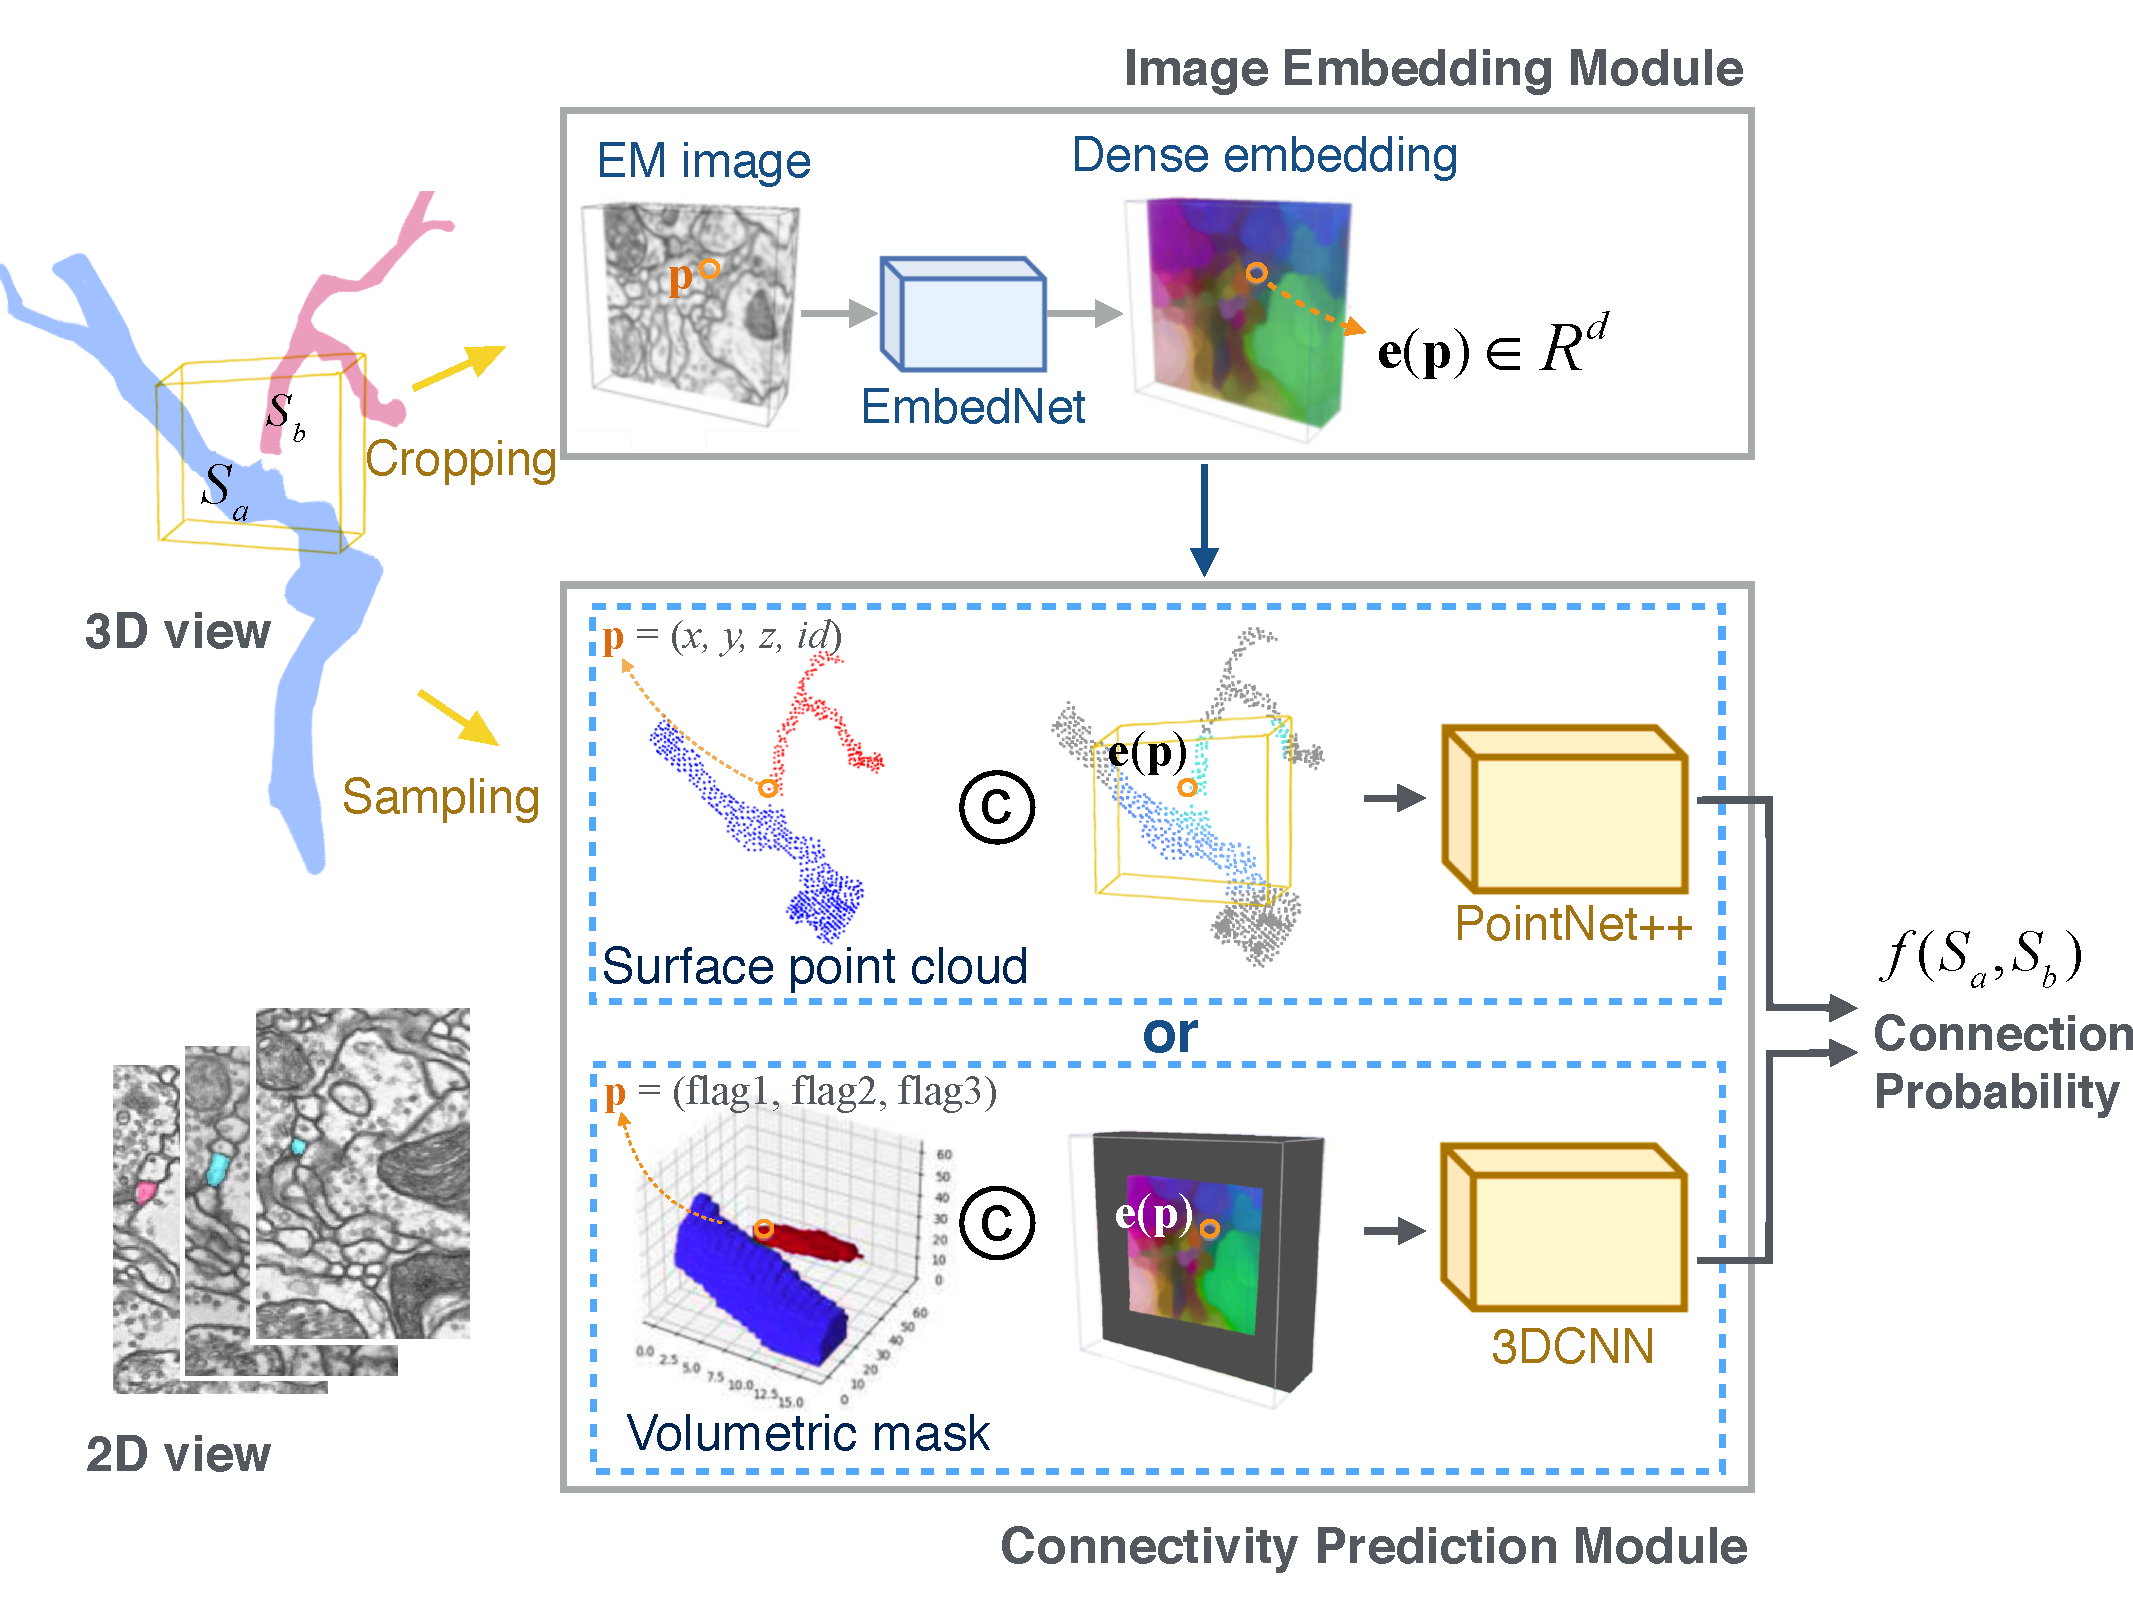
\includegraphics[width=0.48\textwidth]{figs/3Dmodel.pdf}
    \caption{Our connectivity prediction framework fuses local volumetric image features extracted by the EmbedNet with 3D morphology, optionally represented by point cloud or volumetric masks.}% 
    \label{fig:3Dmodel}
\end{figure}

Consequently, we collect the entire bridging edge set from $23,769$ proofread neurons.
The average count of bridging edges per neuron is 810. 
%
For each bridging edge $edge(\mathbf{v}_i, \mathbf{v}_j)$, assuming ${\mathbf{c}}_{i,j}$ is the midpoint of $\mathbf{v}_i$ and $\mathbf{v}_j$, we add random shift to the coordinate of ${\mathbf{c}}_{i,j}$ and obtain ${\hat{\mathbf{c}}}_{i,j}$ as the estimated truncated point. 
The segment pair $(S_a, S_b)$ is annotated as a positive connecting pair ($f(S_a, S_b)=1$).
Any segment $S_c$ that is located in the cube of size $H\times W\times D$ centered at ${\hat{\mathbf{c}}}_{i,j}$ and $S_c \neq S_b$ is labeled with $S_a$ as a negative pair ($f(S_a, S_c)=0$). 


 \subsubsection{Training and Test Block Partition.}
The positive segment pairs across the entire fly brain are partitioned into blocks based on their location in the brain, each spanning a volume size of $26\times 26\times 1\mu m^3$. We select $4,000$ blocks, each of which contains a minimum of $350$ positive segment pairs for training and testing. 
 $1,000$ blocks are selected randomly as the training and validation set for the image embedding network and pairwise connectivity prediction models. The rest $3,000$ blocks are used for testing of connectivity prediction.
 
 

\section{Methods}

\subsection{Problem Formulation}
In crop yield prediction, we denote each county's climatic features by $\mathbf{x}_{c,t}$ and ground-truth crop yield (for a particular crop) by $y_{c,t}\in \mathbb{R}$, where $c$, $t$ represent county and year respectively. Each $\mathbf{x}_{c,t}$ contains four types of features (detailed descriptions of these features can be found in the Experiments section): weather features $\mathbf{x}_{c,t}^w\in \mathbb{R}^{n_w\times 52}$, land surface features $\mathbf{x}_{c,t}^l\in \mathbb{R}^{n_l\times 52}$, soil quality features $\mathbf{x}_{c}^s\in \mathbb{R}^{n_s\times 6}$, and some extra features (e.g. crop production index) $\mathbf{x}_{c}^e\in \mathbb{R}^{n_e}$. Namely, $\mathbf{x}_{c,t}=(\mathbf{x}_{c,t}^w, \mathbf{x}_{c,t}^l, \mathbf{x}_{c}^s, \mathbf{x}_{c}^e)$. We denote the number of weather, land surface, soil quality, and extra variables as  $n_w, n_l, n_s, n_e$ respectively. Among these features, $\mathbf{x}_{c,t}^w, \mathbf{x}_{c,t}^l$ change both spatially and temporally, while $\mathbf{x}_{c}^s, \mathbf{x}_{c}^e$ are county-specific and remain stable over time. The goal is to predict $y_{c,t}$ given $\mathbf{x}_{c,t}$. Recent work \cite{khaki2020cnn} also showed features from past years can help with the prediction, so we reformulate our task as predicting $y_{c,t}$ with $\{\mathbf{x}_{c,t},\mathbf{x}_{c,t-1},...,\mathbf{x}_{c,t-\Delta t}\}$. $\Delta t$ is the length of year dependency. If $\Delta t=0$, the model will not consider features from prior years. 

\subsection{Per-Year Embedding Extraction}
Regardless of whether the models use historical features or not, the first step is always to extract an embedding for each year from $\mathbf{x}_{c,t}$. Then a prediction can be made based on the embedding from the current year or the embeddings from the last few years.

The four types of features $\mathbf{x}_{c,t}^w, \mathbf{x}_{c,t}^l, \mathbf{x}_{c}^s, \mathbf{x}_{c}^e$ have different structures. Using a uniform neural network to extract the embedding may not effectively exploit the structure in the raw data. For example, weekly features $\mathbf{x}_{c,t}^w, \mathbf{x}_{c,t}^l$ naturally incorporate a temporal order, but county-specific soil features $\mathbf{x}_{c}^s$ do not change temporally and are measured at different depths underground. Therefore, we use separate neural networks to process the differently structured-parts from $\mathbf{x}_{c,t}$:
\begin{equation}
\label{eq:cnn}
\begin{aligned}
&\mathbf{h}_{c,t}^{wl}=f_{wl}(\mathbf{x}_{c,t}^w, \mathbf{x}_{c,t}^l) \\
&\mathbf{h}_{c}^s=f_s(\mathbf{x}_{c}^s) \\
&\mathbf{h}_{c,t}=(\mathbf{h}_{c,t}^{wl}, \mathbf{h}_c^s, \mathbf{x}_{c}^e)
\end{aligned}
\end{equation}
$f_{wl}(\cdot)$ handles the features that vary over time. Since land surface features like soil moisture from $\mathbf{x}_{c,t}^l$ are weekly data closely related to weather, we concatenate $\mathbf{x}_{c,t}^l$ and $\mathbf{x}_{c,t}^w$ before further passing to $f_{wl}$. Given the temporal order, an RNN or a CNN can be used for $f_{wl}$ to facilitate information aggregation along the time axis. On the other hand, $f_s(\cdot)$ aggregates information along soil depths. We use CNN as the architecture for $f_s$. $\mathbf{x}_{c}^e$ only contains six scalar values, so we directly pass it to the output embedding. The final embedding $\mathbf{h}_{c,t}$ is the concatenation of $\mathbf{h}_{c,t}^{wl}, \mathbf{h}_c^s, \mathbf{x}_{c}^e$.


\begin{figure*}[t]
\centering
\begin{minipage}[c]{7cm}
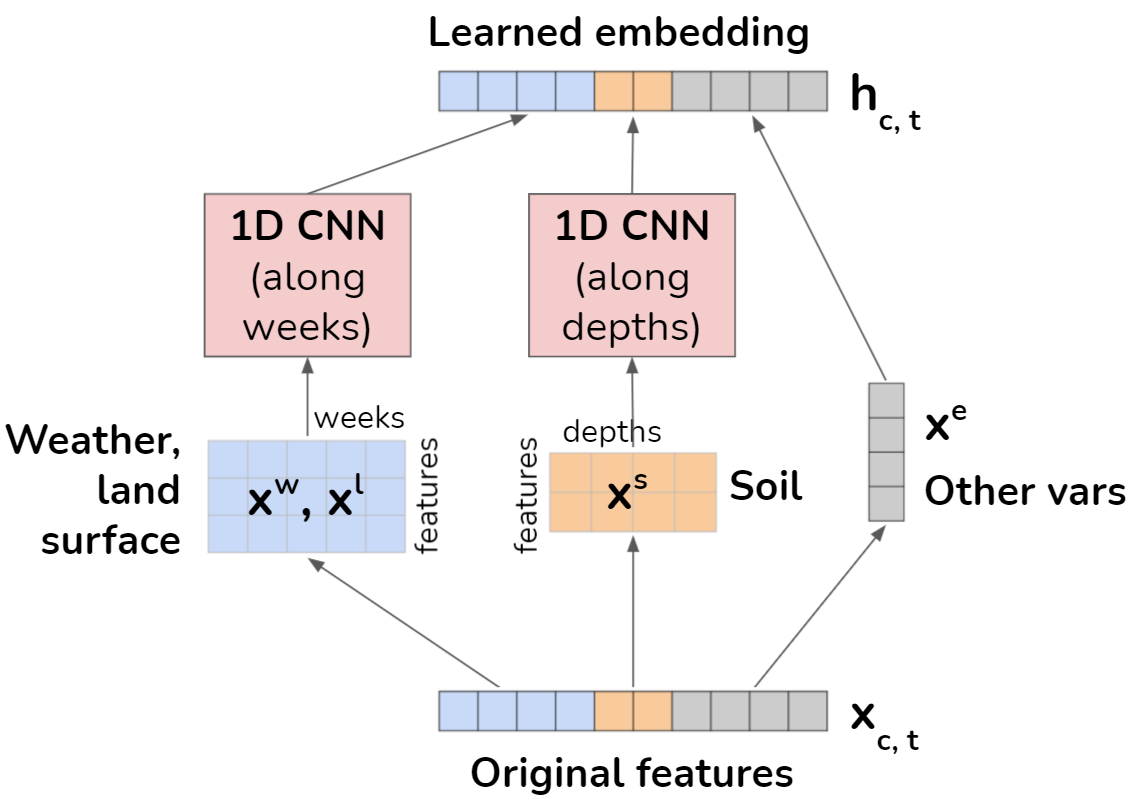
\includegraphics[width=6.9cm]{figs/cnn.png}
\label{fig:cnn}
\end{minipage}
\begin{minipage}[c]{10cm}
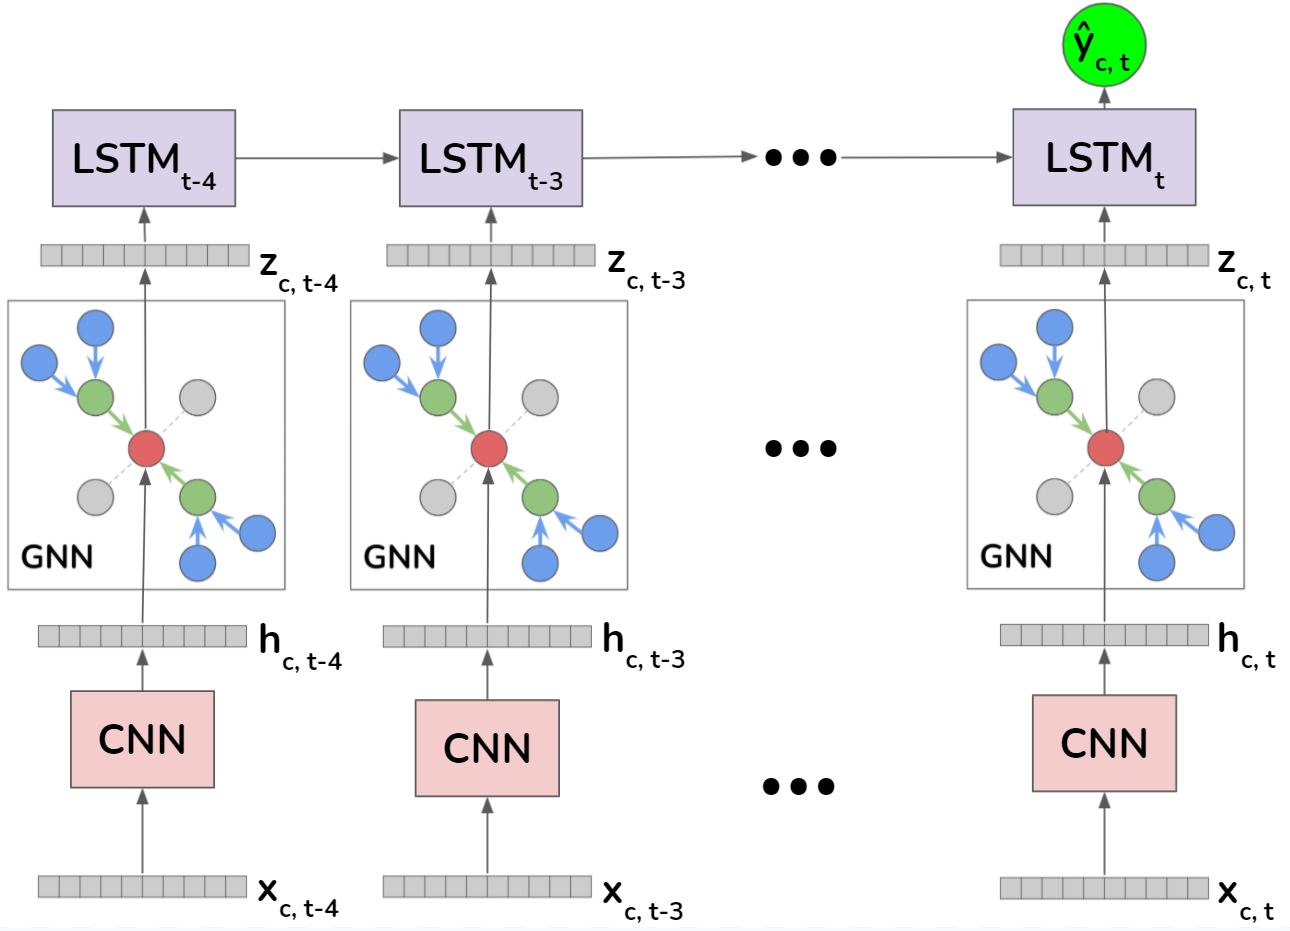
\includegraphics[width=9.9cm]{figs/gnn-rnn.png}
\label{fig:gnn-rnn}
\end{minipage}
\caption{\textbf{Left}: The CNN model used for per-year embedding extraction. \textbf{Right}: Our overall GNN-RNN framework. For each county $c$ and year $t'$, the CNN extracts an embedding $\mathbf{h}_{c, t'}$. Then we apply a GNN to refine each year's embedding by aggregating information from neighboring counties, producing a new embedding $\mathbf{z}_{c, t'}$. Finally, an LSTM processes the embeddings from each year and outputs the yield prediction $\widehat{y}_{c, t}$.}
\end{figure*}


\subsection{Temporal Dependency}
Though new crops are planted every year and yields primarily depend on climatic factors within one year, it has been observed that the trend and variations captured by recent history can be very informative for prediction \cite{khaki2020cnn}. For example, crop yields have tended to increase over the past few decades due to improvements in technology and genetics \cite{ortiz2018another}. While data on the underlying technological improvement is unavailable \cite{khaki2020cnn}, we can observe recent trends in crop yield. Our per-year embedding extraction makes it easy to incorporate  historical knowledge. All we need is an RNN that reads the per-year embeddings from the current year and several prior years. The output from the last time step would be our prediction for the crop yield of the current year: 
\begin{equation}
\label{eq:rnn}
\begin{aligned}
\widehat{y}_{c,t}=r(\mathbf{h}_{c,t-\Delta t}, ..., \mathbf{h}_{c,t-1}, \mathbf{h}_{c,t})
\end{aligned}
\end{equation}
where $r(\cdot)$ is an RNN, and $\mathbf{h}_{c,t'}$ is the embedding from year $t'$ for county $c$. The model described so far follows the CNN-RNN framework, which has previously been shown to outperform single-year NN models \cite{khaki2020cnn}.


\subsection{Incorporating Geographical Knowledge}
Eq.~\ref{eq:rnn} shows how one can extend the use of embeddings from Eq.~\ref{eq:cnn} temporally. Then a natural question is, Can we take advantage of the embeddings geospatially as well? Intuitively, if a county has good yields, nearby counties tend to have good yields as well. The weather and soil conditions should also transition smoothly across the continent. The additional features from neighboring counties could boost the prediction if used properly. A recent success in COVID-19 forecasting \cite{kapoor2020examining} with similar insights could further support incorporating geographical knowledge, where the graph-based representation learning greatly improves case prediction. 

\subsubsection{Graph Neural Network}
Graph Neural Network (GNN) \cite{zhou2020graph} is a novel type of neural network proposed to unravel the complicated dependencies inherent in graph-structured data sources.
%GNN allows more flexibility and a wider representation space to embed the node and edge information from the graph for inference.
Given its strong power in representation learning, GNN has demonstrated prominent applications in chemistry \cite{gilmer2017neural}, traffic \cite{cui2019traffic}, biology \cite{fout2017protein}, and computer vision \cite{satorras2018few} with sophisticated model architectures \cite{kipf2016semi,hamilton2017inductive,velivckovic2017graph}. Formally, a graph is denoted by $G=(V,E)$ where $V$ is the set of nodes and $E$ is the set of edges between nodes. In our crop yield prediction task, each node is a county. $E$ is represented as a symmetric adjacency matrix $A\in \{0,1\}^{N\times N}$ where $A_{i,j}=1$ if two counties $v_i, v_j\in V$ border and $A_{i,j}=0$ otherwise. $N$ is the total number of counties. Each node is associated with $\mathbf{x}_{c,t}$ for every year. 

\subsubsection{GraphSAGE} 
A popular GNN model, GraphSAGE, \cite{hamilton2017inductive} is a general framework that leverages node feature information and learns node embeddings through aggregation from a node's local neighborhood. Unlike many other methods based on matrix factorization and normalization \cite{jia2020residual}, GraphSAGE simply aggregates the features from a local neighborhood, and is thus less computationally expensive. The features can be aggregated from a different number of hops or search depth. Therefore the model often generalizes better. GraphSAGE is suitable for crop yield prediction because most counties only border a few others and the adjacency matrix is sparse. It also provides flexible aggregation methods.

Formally, for the $l$-th layer of GraphSAGE, 
\begin{equation}
\label{eq:gnn}
\begin{aligned}
&\mathbf{a}_{c,t}^{(l)} = g_l(\{\mathbf{z}_{c',t}^{(l-1)},\forall c'\in\mathcal N(c)\})\\
&\mathbf{z}_{c,t}^{(l)} = \sigma(\mathbf{W}^{(l)}\cdot (\mathbf{z}_{c,t}^{(l-1)}, \mathbf{a}_{c,t}^{(l)}))
\end{aligned}
\end{equation}
where $\mathbf{z}_{c,t}^{(0)}=h_{c,t}$ from Eq.~\ref{eq:cnn}, and $l\in\{0,1,...,L\}$. $\mathcal N(c)=\{c', \forall A_{c,c'}=1\}$ is the set of neighboring counties for $c$. The aggregation function for the $l$-th layer is denoted $g_l(\cdot)$, which could be mean, pooling, or graph convolution (GCN) function. In practice, we found mean or pooling are effective and computationally efficient. $\mathbf{a}_{c,t}^{(l)}$ is the aggregated embedding from the bordering counties. We concatenate $\mathbf{a}_{c,t}^{(l)}$ with the last layer's embedding $\mathbf{z}_{c,t}^{(l-1)}$ before the transformation using $\mathbf{W}^{(l)}$. $\sigma(\cdot)$ is a non-linear function.

\subsubsection{GNN-RNN}
The output embedding from GNN's last layer $\mathbf{z}_{c,t}^{(L)}$ thus extracts the information (e.g., weather, soil) from the whole local neighborhood for year $t$. To integrate the historical knowledge, we can do the same as in Eq.~\ref{eq:rnn}, by taking the GNN output embeddings from prior years:
\begin{equation}
\label{eq:gnn-rnn}
\begin{aligned}
\widehat{y}_{c,t}=r(\mathbf{z}_{c,t-\Delta t}^{(L)}, ..., \mathbf{z}_{c,t-1}^{(L)}, \mathbf{z}_{c,t}^{(L)})
\end{aligned}
\end{equation}
where $\mathbf{z}_{c,t'}^{(L)}$ is the GNN embedding from year $t'$.

\subsubsection{Loss Function}
We use log-cosh function as our objective:
\begin{equation}
\begin{aligned}
L(\widehat{y}_{c,t}, y_{c,t})=\log(\text{cosh}(\widehat{y}_{c,t}-y_{c,t}))
\end{aligned}
\end{equation}
Log-cosh works similarly to mean square error, but is not as strongly affected by the occasional wildly incorrect prediction. It is also twice differentiable everywhere. Mini-batch training is adopted during optimization. Batch loss is the average log-cosh loss of all samples in a batch. 


\section{Background \& Related Work\label{sec:related}}

\subsection{Algorithmic Accountability}
As algorithmic approaches replace and supplant human decisions across society, researchers have pointed out the importance of holding algorithms accountable \citep{Gillespie2014,Diakopoulos2015,Garfinkel2017}. One way to do this is the ``algorithm audit,'' which derives its name and approach from longstanding methods in the social sciences designed to detect discrimination \citep{Sandvig2014}. For example, algorithm audits have exposed discrimination in image search algorithms \citep{Kay}, Google auto-complete \citep{Baker2013}, dynamic pricing algorithms \citep{Chen2016}, automated facial analysis \citep{Buolamwini2018}, and word embeddings \citep{Caliskan2017}. Of particular relevance to our work are audit studies focusing on news intermediaries which aggregate, filter, and sort news content from primary publishers.

\subsection{Auditing Intermediaries}
Examples of algorithmic news intermediaries include social media websites (e.g. Facebook, Twitter, reddit), search engines (e.g. Google, Bing), and news aggregation websites (e.g. Google News). On each of these platforms, algorithms select and sort content for millions of users, thus wielding significant power as algorithmic gatekeepers. This content moderation has attracted critical attention \citep{Gillespie2018}, and spurred some researchers to audit intermediaries and check for discrimination, diversity, or filter-bubble effects.

\subsubsection{Social Media}
In the case of social media, \citet{Bakshy} investigated Facebook's News Feed, finding that user choices (e.g., click history, visit frequency) played a stronger role than News Feed's algorithmic ranking when it came to helping users encounter ideologically cross-cutting content. A 2009 study of Twitter showed that trending topics were more than 85\% news-oriented \citep{Kwak2010}. However, because of the high churn rate, trending topics can exhibit temporal coverage bias depending on when users visit the site \citep{Chakraborty2015}.

\subsubsection{Web Search}
As the most popular platform for online search, Google has been the subject of numerous audit studies, some of which reveal discriminatory results. For example, Google's autocomplete feature was shown to exhibit gender and racial biases \citep{Baker2013}, and its image search was shown to systematically underrepresent women \citep{Kay}. Other audits show that user-generated content such as Stack Overflow, Reddit, and particularly Wikipedia play a critical role in Google's ability to satisfy search queries \cite{Vincent2019}

Several studies have investigated potential political bias in Google's search results \citep{Robertson2018,Diakopoulos,Epstein2017}, however, further research is needed to understand the extent and causes of apparent biases. For example, Google's search algorithms may increase exposure to particular news sources (with left-leaning audiences) due to freshness, relevance, or greater overall abundance of content on the web \citep{Trielli}.

Some studies have also investigated Google for creating virtual echo chambers, which may affect democratic processes. While concern has mounted over the search engine's filter-bubble effects \citep{Pariser}, studies have thus far found limited supporting evidence for the phenomenon \citep{Puschmann2018,Flaxman,Hannak2013,Robertson2018}. An analysis of more than 50,000 online users in the United States showed that the search engine can actually ``increase an individual's exposure to material from his or her less preferred side of the political spectrum'' \citep{Flaxman}. Still, some search results may vary with respect to location \citep{Kliman-Silver2015}, an effect that has the potential to create geolocal filter bubbles. %\citep{Hannak2017} examine 200 Google webs earch users and show that ``on average, 11.7\% of results show differences due to personalization.'' Similarly, \citep{Robertson2018} found minimal evidence for the filter bubble hypothesis.

\subsubsection{Google News}
As early as 2005, researchers zeroed in on Google's news system to assess potential bias in the platform \citep{Ulken2005,Schroeder2005}, showing that even shortly after its introduction, scholars were troubled by the platform's potential effects on journalism and the public at large. For example, the Associated Press was concerned that Google used their content without providing compensation \citep{Gaither2005}, and early on, Google News was suspected to have a conservative bias \citep{Ulken2005}.

Google News still attracts critical attention more than a decade later, but concerns have shifted towards the possibility of filter bubbles (as was the case with Google's search engine). Two studies in particular have addressed such concerns: \citet{Haim2018} tested for personalization with manually-created user profiles, and \citet{Nechushtai2019} did so with real-world users. The former study discovered ``minor effects'' on content diversity from both explicit personalization (from user-stated preferences) and implicit personalization (using inferences from observed online behavior). \citet{Nechushtai2019} showed that users with different political leanings and locations ``were recommended very similar news,'' but their study presented a separate concern: just five news outlets accounted for 49\% of the 1,653 recommended news stories. This source concentration highlights the multifaceted implications of news aggregators, which we return to later.


\subsubsection{Apple News}
Apple News has begun to attract the interest of various stakeholders in industry and research. The New York Times wrote about the app in October 2018 \citep{Nicas2018}, focusing on Apple's ``radical approach'' of using humans to curate content instead of just algorithms. Despite its growth, monetization on the platform has thus far proven difficult and drawn criticism \citep{Davies2017,Dotan2018}. Slate reports that it takes 6 million page views in the Apple News app to generate the same advertising revenue as 50,000 page views on its website -- a more than hundredfold difference \citep{Oremus2018}.

A study of Apple News' editorial curation choices in June 2018 analyzed tweets and email newsletters from the editors, finding that larger publishers appeared far more often \citep{Brown2018}. In a followup study, screen recordings captured the Top Stories section in the United Kingdom to collect 1,031 total articles, 75\% of which came from just six publishers \citep{Brown2018a}. This paper builds on and adds to these studies in two important ways. First, we design and use a method for \textit{fully automated data collection}, rather than relying on manual coding of screen recordings. This method allows us to collect both Top Stories and Trending Stories in the United States, whereas \citep{Brown2018a} collected only Top Stories in the United Kingdom. Second, we examine mechanical aspects of Apple News in addition to examining content. By investigating mechanisms such as adaptation and update frequency, we reveal several intriguing design choices and curation patterns within the app.

\section{Experiments}



We compare 11 representative machine learning models, including GNN and GNN-RNN, on US county-level crop yields for corn and soybean. We evaluate performance on three metrics: RMSE, $R^2$, and correlation coefficient. Given a test year $t$, we use year $t-1$ for validation and all the prior years for training. For example, if the test year is 2019, we train on data from years 1981-2017 (inclusive), validate on 2018 crop yields, and test on 2019 crop yields.

\subsection{Dataset Details}

% NOte: see dataset_OLD.tex for more detailed text, if we need it in the future

Crop yield labels for corn and soybean are available from the USDA Crop Production Reports \cite{usda2013national} for numerous counties in the US. Not all counties report data in every year, but the coverage is still quite comprehensive. For example, for corn, all years between 1981 and 2003 have over 2,000 counties across $41$ states reporting data. We train and evaluate our model on all counties where yield data is available. (When computing the loss, we ignore counties that do not have yield labels for that year.)

We use a variety of climate, land surface, and soil quality variables as input features; these features are available for almost all counties in the contiguous 48 US states (3,107 counties in total\footnote{The only exception is Nantucket County, Massachusetts, where land surface model data is missing, since it is an offshore island. Also note that some counties have feature data but not label (yield) data. Only the GNN and GNN-RNN models can make use of these unlabeled county features.}). We draw 7 weather features from the PRISM climate mapping system \cite{daly2013prism}: precipitation, min/mean/max temperature, min/max vapor pressure deficit, and mean dewpoint temperature. These features are available at a $4 \times 4$ km grid for each day. 

We acquire 16 land surface features from the North American Land Data Assimilation System (NLDAS) \cite{xia2012continental}, which is a large-scale land surface model that closely simulates land surface parameters. These features include soil moisture content, moisture availability, and soil temperature (all at various soil depths), as well as observed weather variables such as wind speed and humidity. These variables are available at a $0.125 \times 0.125$ degree ($\sim 14$ km) spatial resolution, every hour. 

%We aggregate the hourly data to daily, and aggregate the grid to the county level in the same way as PRISM. 


% We acqui  gSSURGO dataset \cite{soil2019gridded} provides abundant survey-collected features regarding the soil composition and quality of an area. These gridded features are available at a 30-meter spatial resolution, and \emph{do not change over time}.

Soil quality features were acquired from the Gridded Soil Survey Geographic Database (gSSURGO) \cite{soil2019gridded}, at a $30 \times 30$ meter resolution. These features include available water capacity, bulk density, and electrical conductivity, pH, and organic matter.
% We used 20 features that are available at 6 different soil depth levels, as well as 6 ``extra'' features (such as crop productivity indices) that are not depth-dependent. 
Unlike the weather and land surface features, the gSSURGO soil quality features are fixed and \emph{do not change over time}. In addition to the raw features, we use the raw sand, silt, and clay percentages to compute the ``soil texture type'' of each pixel based on the Natural Resources Conservation Service Soil Survey's classification scheme \cite{soiltexture}, and then compute the fraction of each county occupied by each soil texture type. In total, we have a total of 20 gSSURGO variables that are depth-dependent (so there are values for 6 different soil depth levels), and 6 ``extra'' variables which are not depth-dependent (such as crop productivity indices). Finally, as in \cite{khaki2020cnn}, we use the average crop yield (over all counties) of the previous year as an additional input feature, to capture the increasing trend in crop yield over time. A full list of the features can be found in the Appendix.

%Again, we aggregate these features to the county level using the weighted-average technique, only considering pixels that are cropland/grassland/pasture.
% The North American Land Data Assimilation System (NLDAS) \cite{xia2012continental} is a large-scale land surface model that closely simulates land surface parameters. We collect 16 features from this dataset, including several ``forcing'' weather variables, as well as soil moisture, moisture availability, and soil temperature at multiple soil depths. These data are originally available at a $0.125 \times 0.125$ degree (roughly $14$ km) spatial resolution, and an hourly temporal resolution. We aggregate the hourly data to daily, and aggregate the grid to the county level in the same way as PRISM. 


All of these datasets were originally available as gridded raster data at a variety of spatial resolutions. We aggregated each feature to the county level by computing the weighted average of the variable over all grid cells that overlap with the county. Each grid cell is weighted by the percentage of the cell that lies inside the county, multiplied by the percentage of that grid cell which is cropland, pasture, or grassland; the land cover percentages are computed using the National Land Cover Database \cite{nlcd}. In addition, the time-dependent variables (weather and land surface) were aggregated from daily to weekly frequency to make the prediction task more tractable.

%Figure \ref{aggregating_to_county} shows an example of the process we use to aggregate gridded features to the county level.

% \begin{figure}[t]
% \centering
% \includegraphics[width=0.75\columnwidth]{figs/nldas.png}
% \includegraphics[width=0.75\columnwidth]{figs/nldas_SOILM_layer1_19810101_county.png}
% \caption{Example of aggregating features to county level. \\
% \textbf{(a)} raw raster of soil moisture from NLDAS. \\
% \textbf{(b)} Percentage cropland/grassland/pasture (used to compute grid cell weights).\\
% \textbf{(c)} the county-level values we generated. \textbf{make bigger, make size of figures consistent}}
% \label{aggregating_to_county}
% \end{figure}

\subsection{Compared Methods}

We consider two types of methods: \textbf{(a) single-year methods} that only use features from year $t$ to predict yield for the same year $t$, and \textbf{(b) 5-year methods} that use features from a 5-year series (years $\{t-4, t-3, \dots, t\}$) to predict yield for year $t$.

\textbf{Single-year methods.} We first consider methods that only use a single year of data to make predictions, to provide a fair comparison to the single-year GNN. For non-deep baseline methods, we select lasso, ridge regressor and gradient boosting regressor. For these methods, we flatten all the features from the entire year into a single feature vector, ignoring the temporal and soil-depth structure in the data.
Next, we tried three baseline deep learning architectures for $f_{wl}(\cdot)$: LSTM \cite{hochreiter1997long}, GRU \cite{chung2014empirical}, and 1-D CNN \cite{kalchbrenner2014convolutional}. All of these methods process the weekly time-series of weather and land surface data within the year. We compare these methods with our single-year GNN model (Eq. \ref{eq:gnn}), which incorporates geospatial context in making predictions.
 
\textbf{5-year methods.} For history-dependent models, we follow \cite{khaki2020cnn} by considering a 5-year dependency for a consistent and fair comparison. Two baseline models using LSTM and GRU respectively handle the raw inputs $\{\mathbf{x}_{c,t-\Delta t}, ...,\mathbf{x}_{c,t}\}$ directly with $r(\cdot)$. Specifically, they flatten the features \emph{for each year} into a single vector (disregarding the weekly structure of the weather data or the depth structure of the soil data), and then feed the 5 year-vectors into the LSTM or GRU. The most recent CNN-RNN model \cite{khaki2020cnn} pre-processes the raw features with a CNN (choosing CNN for $f_{wl}(\cdot)$) and then uses a LSTM to model the sequence embeddings as described in Eq. \ref{eq:rnn}. Finally, the GNN-RNN model proposed in this paper (Eq. \ref{eq:gnn-rnn}) still uses a CNN for $f_{wl}(\cdot)$ to encode the raw features into an embedding for each year, then uses the GNN to refine the embeddings using information from the county's spatial context, and then passes those embeddings into an LSTM.

% Two additional methods proposed in this paper are single year GNN (Eq. \ref{eq:gnn}) and GNN-RNN (Eq. \ref{eq:gnn-rnn}).


\subsection{Evaluation Metrics}
We evaluate all methods on three popular metrics for regression: root mean square error (RMSE), the coefficient of determination ($R^2$), Pearson correlation coefficient (Corr). RMSE and $R^2$ tell us how well a regression model can predict the value of the response variable in absolute terms and percentage terms respectively. Note that our RMSE figures are expressed in units of the standard deviation of that crop's yield (across all years). Corr is essentially a normalized measurement of the covariance between two sets of data, and captures the strength of the linear correlation between true and predicted values. See Appendix for formal definitions.


\begin{table*}[tb]
\centering
\subfloat[2018 corn results]{
\begin{tabular}{|l|c|c|c|} \hline
\textbf{Method} & \textbf{RMSE} & \textbf{$R^2$} & \textbf{Corr} \\ \hline
% \multicolumn{4}{|l|}{\textbf{1-year methods}} \\ \hline
lasso 1y & 0.7846 & 0.3839 & 0.7778 \\
ridge 1y & 0.9255 & 0.1428 & 0.7626 \\
gradient-boosting 1y & 0.7402 & 0.4516 & 0.7794 \\
gru 1y & 0.5938 & 0.6472 & 0.8158 \\
lstm 1y & 0.6146 & 0.6220 & 0.8303 \\
cnn 1y & 0.5824 & 0.6606 & 0.8235 \\ \hdashline
gnn 1y \textbf{(ours)} & \textbf{0.4846} & \textbf{0.7517} & \textbf{0.8759} \\
\fontsize{9}{10}\selectfont
\std{std} & \std{0.0097} & \std{0.0100} & \std{0.0019}
\fontsize{10}{10}\selectfont\\
\hline %\Xhline{1.5pt} 
% \multicolumn{4}{|l|}{\textbf{5-year methods}} \\ \hline
gru 5y & 0.6765 & 0.5419 & 0.8194 \\
lstm 5y & 0.6542 & 0.5716 & 0.8060 \\
cnn-rnn 5y & 0.5511 & 0.6936 & 0.8425 \\ \hdashline
gnn-rnn 5y \textbf{(ours)} & \textbf{0.4900} & \textbf{0.7595}  & \textbf{0.8731} \\ 
\fontsize{9}{10}\selectfont
\std{std} & \std{0.0191} & \std{0.0186} & \std{0.0092} 
\fontsize{10}{10}\selectfont \\ \hline
\end{tabular}
} \qquad
\subfloat[2019 corn results]{
\begin{tabular}{|l|c|c|c|} \hline
\textbf{Method} & \textbf{RMSE} & \textbf{$R^2$} & \textbf{Corr} \\ \hline
lasso 1y & 0.6838 & 0.3122 & 0.6715 \\
ridge 1y & 0.7081 & 0.2623 & 0.6723 \\
gradient-boosting 1y & 0.7345 & 0.2064 & 0.6857 \\
gru 1y & 0.5890 & 0.4897 & 0.7381 \\
lstm 1y & 0.6245 & 0.4262 & 0.7096 \\
cnn 1y & 0.5572 & 0.5432 & 0.7384 \\ \hdashline
gnn 1y \textbf{(ours)} & \textbf{0.4930} & \textbf{0.6286} & \textbf{0.8011} \\
\fontsize{9}{10}\selectfont
\std{std} & \std{0.0068} & \std{0.0102} & \std{0.0037}
\fontsize{10}{10}\selectfont\\ \hline
gru 5y & 0.5279 & 0.5900 & 0.7785 \\
lstm 5y & 0.5311 & 0.5849 & 0.7821 \\
cnn-rnn 5y & 0.5212 & 0.5842 & 0.7868 \\ \hdashline
gnn-rnn 5y \textbf{(ours)} & \textbf{0.4677} & \textbf{0.6782} & \textbf{0.8272} \\
\std{std} & \std{0.0035} & \std{0.0049} & \std{0.0038} \\ \hline
\end{tabular}
} \\
\subfloat[2018 soybean results]{
\begin{tabular}{|l|c|c|c|} \hline
\textbf{Method} & \textbf{RMSE} & \textbf{$R^2$} & \textbf{Corr} \\ \hline
lasso 1y & 0.6226 & 0.6090 & 0.7912 \\
ridge 1y & 0.7633 & 0.4125 & 0.7550 \\
gradient-boosting 1y & 0.6686 & 0.5492 & 0.7986 \\
gru 1y & 0.6376 & 0.5932 & \textbf{0.8356} \\
lstm 1y & 0.6459 & 0.5825 & 0.8129 \\
cnn 1y & 0.6584 & 0.5661 & 0.7988 \\ \hdashline
gnn 1y \textbf{(ours)} & \textbf{0.5637} & \textbf{0.6794} & 0.8273 \\
\fontsize{9}{10}\selectfont
\std{std} & \std{0.0144} & \std{0.0163} & \std{0.0095}
\fontsize{10}{10}\selectfont\\ \hline
 % \Xhline{1.5pt}
gru 5y & 0.6094 & 0.6254 & 0.8218 \\
lstm 5y & 0.5430 & 0.7026 & 0.8459 \\
cnn-rnn 5y & 0.5647 & 0.6784 & \textbf{0.8650} \\ \hdashline
gnn-rnn 5y \textbf{(ours)} & \textbf{0.5333} & \textbf{0.7129} & 0.8591 \\ 
\fontsize{9}{10}\selectfont
\std{std} & \std{0.0194} & \std{0.0206} & \std{0.0049} 
\fontsize{10}{10}\selectfont
\\ \hline

\end{tabular}
} \qquad
\subfloat[2019 soybean results]{
\begin{tabular}{|l|c|c|c|} \hline
\textbf{Method} & \textbf{RMSE} & \textbf{$R^2$} & \textbf{Corr} \\ \hline
lasso 1y & 0.5731 & 0.6137 & 0.8089 \\
ridge 1y & 0.6069 & 0.5668 & 0.7944 \\
gradient-boosting 1y & 0.6802 & 0.4558 & 0.7899 \\
gru 1y & 0.5742 & 0.5150 & 0.7569 \\
lstm 1y & 0.5907 & 0.4867 & 0.7195 \\
cnn 1y & 0.5699 & 0.5222 & 0.7385 \\ \hdashline
gnn 1y \textbf{(ours)} & \textbf{0.4916} & \textbf{0.7148} & \textbf{0.8505} \\
\fontsize{9}{10}\selectfont
\std{std} & \std{0.0335} & \std{0.0395} & \std{0.0165}
\fontsize{10}{10}\selectfont \\ \hline
gru 5y & 0.5751 & 0.6109 & 0.8158 \\
lstm 5y & 0.5512 & 0.6427 & 0.8156 \\
cnn-rnn 5y & 0.5365 & 0.6615 & 0.8423 \\ \hdashline
gnn-rnn 5y \textbf{(ours)}  & \textbf{0.4745} & \textbf{0.7349} & \textbf{0.8602} \\
% lasso 1y & 0.6838 & 0.3122 & 0.6715 \\
% ridge 1y & 0.7081 & 0.2623 & 0.6723 \\
% gradient-boosting 1y & 0.7345 & 0.2064 & 0.6857 \\
% gru 1y & 0.5890 & 0.4897 & 0.7381 \\
% lstm 1y & 0.6245 & 0.4262 & 0.7096 \\
% cnn 1y & 0.5572 & 0.5432 & 0.7384 \\
% gnn 1y & \textbf{0.4930} & \textbf{0.6286} & \textbf{0.8011} \\ \Xhline{1.5pt} 
% gru 5y & 0.5751 & 0.6109 & 0.8158 \\
% lstm 5y & 0.5512 & 0.6427 & 0.8156 \\
% cnn-rnn 5y & 0.5212 & 0.5842 & 0.7868 \\ \hline
% gnn-rnn 5y & \textbf{0.4679} & \textbf{0.6777} & \textbf{0.8274} \\
\fontsize{9}{10}\selectfont
\std{std} & \std{0.0160} & \std{0.0179} & \std{0.0076}
\fontsize{10}{10}\selectfont \\ \hline
\end{tabular}
}
\caption{Evaluation results. For RMSE, lower is better; for $R^2$ and Corr, higher is better. We grouped the methods based on whether they use 1 year of data (1y) or 5 years of data (5y) to make predictions.}
\label{results}
\end{table*}



\subsection{Model Details}

For the shallow models (ridge regression, lasso, and gradient boosting regressor), we used scikit-learn's implementations. 

For the baseline single-year models, we evaluated using LSTM, GRU, and CNN as $f_{wl}(\cdot)$ to process the weekly weather and land surface data. For CNN, we used a 1-D CNN similar to the one in \cite{khaki2020cnn}, but we process all weather and land surface parameters together. The CNN contains series of 1D convolutions, ReLUs, and average pooling layers; this sequence is repeated four times.  For all methods that use LSTM or GRU, we used PyTorch's implementation with 64 hidden states.


The same CNN is used as the encoder for the weekly weather and land surface data in the CNN-RNN, GNN, and GNN-RNN models. (We also tried using an LSTM as the encoder for the weekly data for these models, but  this did not improve results.) For all methods except for the 5-year LSTM/GRU, we processed the soil data using another small 1-D CNN (with three convolutional layers, and without average pooling), where the convolutions operate across 6 different soil depths.

%For the CNN-RNN model, the CNNs described earlier are used to encode each year's features into an embedding. Then the embeddings for the five years are passed through an LSTM.

For the simple 5-year baseline models (LSTM and GRU), we fed the flattened feature vectors for each year through an LSTM or GRU, followed by a 2-layer fully connected network.


For the GNN and GNN-RNN models, we used the implementation of GraphSAGE from the dgl library; we used a 2-layer GNN, with edge dropout of 0.1. The adjacency graph of US counties is provided by the US Census Bureau. We used stochastic mini-batch training to train the model, where each layer samples 10 neighbors to receive messages from. We tried different aggregation functions and found that the ``pooling'' approach generally performed best.

%The GNN-RNN model considers a sequence of 5 years; the GNN is applied on every year to refine the embeddings produced by the CNN encoder with information from neighboring counties. Then the embeddings outputted by the GNN are fed into a final LSTM and then a fully-connected layer.

For all methods, we use the Adam optimizer \cite{kingma2014adam}, sometimes with a mild cosine or step decay. We tried learning rates between 1e-5 and 1e-3, used a weight decay of 1e-5 or 1e-4, and a batch size of 32, 64, or 128. We trained the model  for 100 to 200 epochs (until the validation loss clearly stopped improving). We chose the epoch and hyperparameter setting that produced the lowest RMSE on the validation year (the year before the test year).  We ran the GNN and GNN-RNN models 3 times with different random seeds to evaluate the variance in the results. The Appendix contains more details about hyperparameters. 


%\junwen{Just for GNN-RNN (required by submission checklist): (1) The number of algorithm runs used to compute each reported result. (2) Analysis of experiments goes beyond single-dimensional summaries of performance.(std) (3) lists all final (hyper-)parameters used for each model. \\ We could put some of these to Appx.}


% \begin{table}[]
% \centering
% % \fontsize{9}{10}\selectfont
% \begin{tabular}{|l|c|c|c|} \hline
% \textbf{Method} & \textbf{RMSE} & \textbf{$R^2$} & \textbf{Corr} \\ \hline
% gru 1y & 0.5890 & 0.4897 & 0.7381 \\
% lstm 1y & 0.6245 & 0.4262 & 0.7096 \\
% cnn 1y & 0.5572 & 0.5432 & 0.7384 \\
% gnn 1y & \textbf{0.4930} & \textbf{0.6286} & \textbf{0.8011} \\ \hline
% lasso 5y & 0.6838 & 0.3122 & 0.6715 \\
% ridge 5y & 0.7081 & 0.2623 & 0.6723 \\
% gradient-boosting 5y & 0.7345 & 0.2064 & 0.6857 \\
% gru 5y & 0.5751 & 0.6109 & 0.8158 \\
% lstm 5y & 0.5512 & 0.6427 & 0.8156 \\
% cnn-rnn 5y & 0.5212 & 0.5842 & 0.7868 \\
% gnn-rnn 5y & \textbf{0.4679} & \textbf{0.6777} & \textbf{0.8274} \\ \hline
% \end{tabular}
% \caption{2019 corn results}
% \label{2019_corn}
% \end{table}

% \begin{table}[]
% \centering
% \fontsize{9}{10}\selectfont
% \begin{tabular}{|l|c|c|c|} \hline
% \textbf{Method} & \textbf{RMSE} & \textbf{$R^2$} & \textbf{Corr} \\ \hline
% gru 1y & 0.6376 & 0.5932 & 0.8356 \\
% lstm 1y & 0.6459 & 0.5825 & 0.8129 \\
% cnn 1y & 0.6584 & 0.5661 & 0.7988 \\
% gnn 1y & \textbf{0.5852} & \textbf{0.6547} & \textbf{0.8175} \\ \hline
% lasso 5y & 0.6226 & 0.6090 & 0.7912 \\
% ridge 5y & 0.7633 & 0.4125 & 0.7550 \\
% gradient-boosting 5y & 0.6686 & 0.5492 & 0.7986 \\
% gru 5y & 0.6094 & 0.6254 & 0.8218 \\
% lstm 5y & 0.5430 & 0.7026 & 0.8459 \\
% cnn-rnn 5y & 0.5647 & 0.6784 & \textbf{0.8650} \\
% gnn-rnn 5y & \textbf{0.5333} & \textbf{0.7129} & 0.8591 \\ \hline
% \end{tabular}
% \caption{2018 soybean results}
% \label{2018_soybean}
% \end{table}

% \begin{table}[]
% \centering
% \fontsize{9}{10}\selectfont
% \begin{tabular}{|l|c|c|c|} \hline
% \textbf{Method} & \textbf{RMSE} & \textbf{$R^2$} & \textbf{Corr} \\ \hline
% gru 1y & 0.5742 & 0.5150 & 0.7569 \\
% lstm 1y & 0.5907 & 0.4867 & 0.7195 \\
% cnn 1y & 0.5699 & 0.5222 & 0.7385 \\
% gnn 1y & \textbf{0.5170} & \textbf{0.6856} & \textbf{0.8299} \\ \hline
% lasso 5y & 0.5731 & 0.6137 & 0.8089 \\
% ridge 5y & 0.6069 & 0.5668 & 0.7944 \\
% gradient-boosting 5y & 0.6802 & 0.4558 & 0.7899 \\
% gru 5y & 0.5751 & 0.6109 & 0.8158 \\
% lstm 5y & 0.5512 & 0.6427 & 0.8156 \\
% cnn-rnn 5y & 0.5365 & 0.6615 & 0.8423 \\
% gnn-rnn 5y & \textbf{0.5091} & \textbf{0.6951} & \textbf{0.8434} \\ \hline
% \end{tabular}
% \caption{2019 soybean results}
% \label{2019_soybean}
% \end{table}



\begin{table}[t]
\centering
\begin{tabular}{|l|c|c|c|} \hline
\textbf{Method} & \textbf{RMSE} & \textbf{$R^2$} & \textbf{Corr} \\ \hline
lstm 1y & 0.6347 & 0.5968 & \textbf{0.8148} \\
cnn 1y & 0.7253	& 0.4736 & 0.7004 \\
gnn 1y \textbf{(ours)} & \textbf{0.5877} & \textbf{0.6543} & 0.8124 \\ \hline
lstm 5y & 0.7004 & 0.5091 & 0.7708 \\
cnn-rnn 5y & 0.6532 & 0.5730 & 0.7732 \\
gnn-rnn 5y \textbf{(ours)} & \textbf{0.5836} & \textbf{0.6591} & \textbf{0.8259} \\ \hline
\end{tabular}
\caption{Early prediction results (2018 corn, after June 1).}
\label{early}
\end{table}

\subsection{Crop Yield Prediction Results}
% Can use https://www.tablesgenerator.com/latex_tables to generate tables from Google sheets


\begin{figure}[bt]
\centering
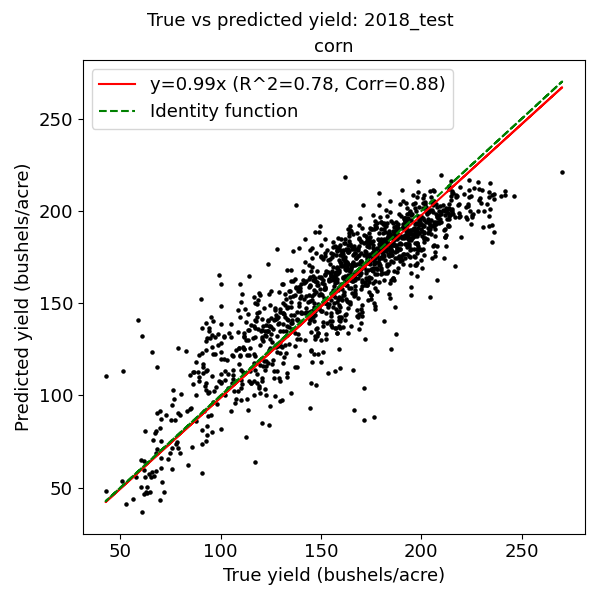
\includegraphics[width=0.8\columnwidth]{figs/true_vs_predicted_scatter_corn_2018_test.png}
\caption{Predicted vs. ground truth corn yields in 2018}
\label{scatter}
\end{figure}

\begin{figure}[tb]
\centering
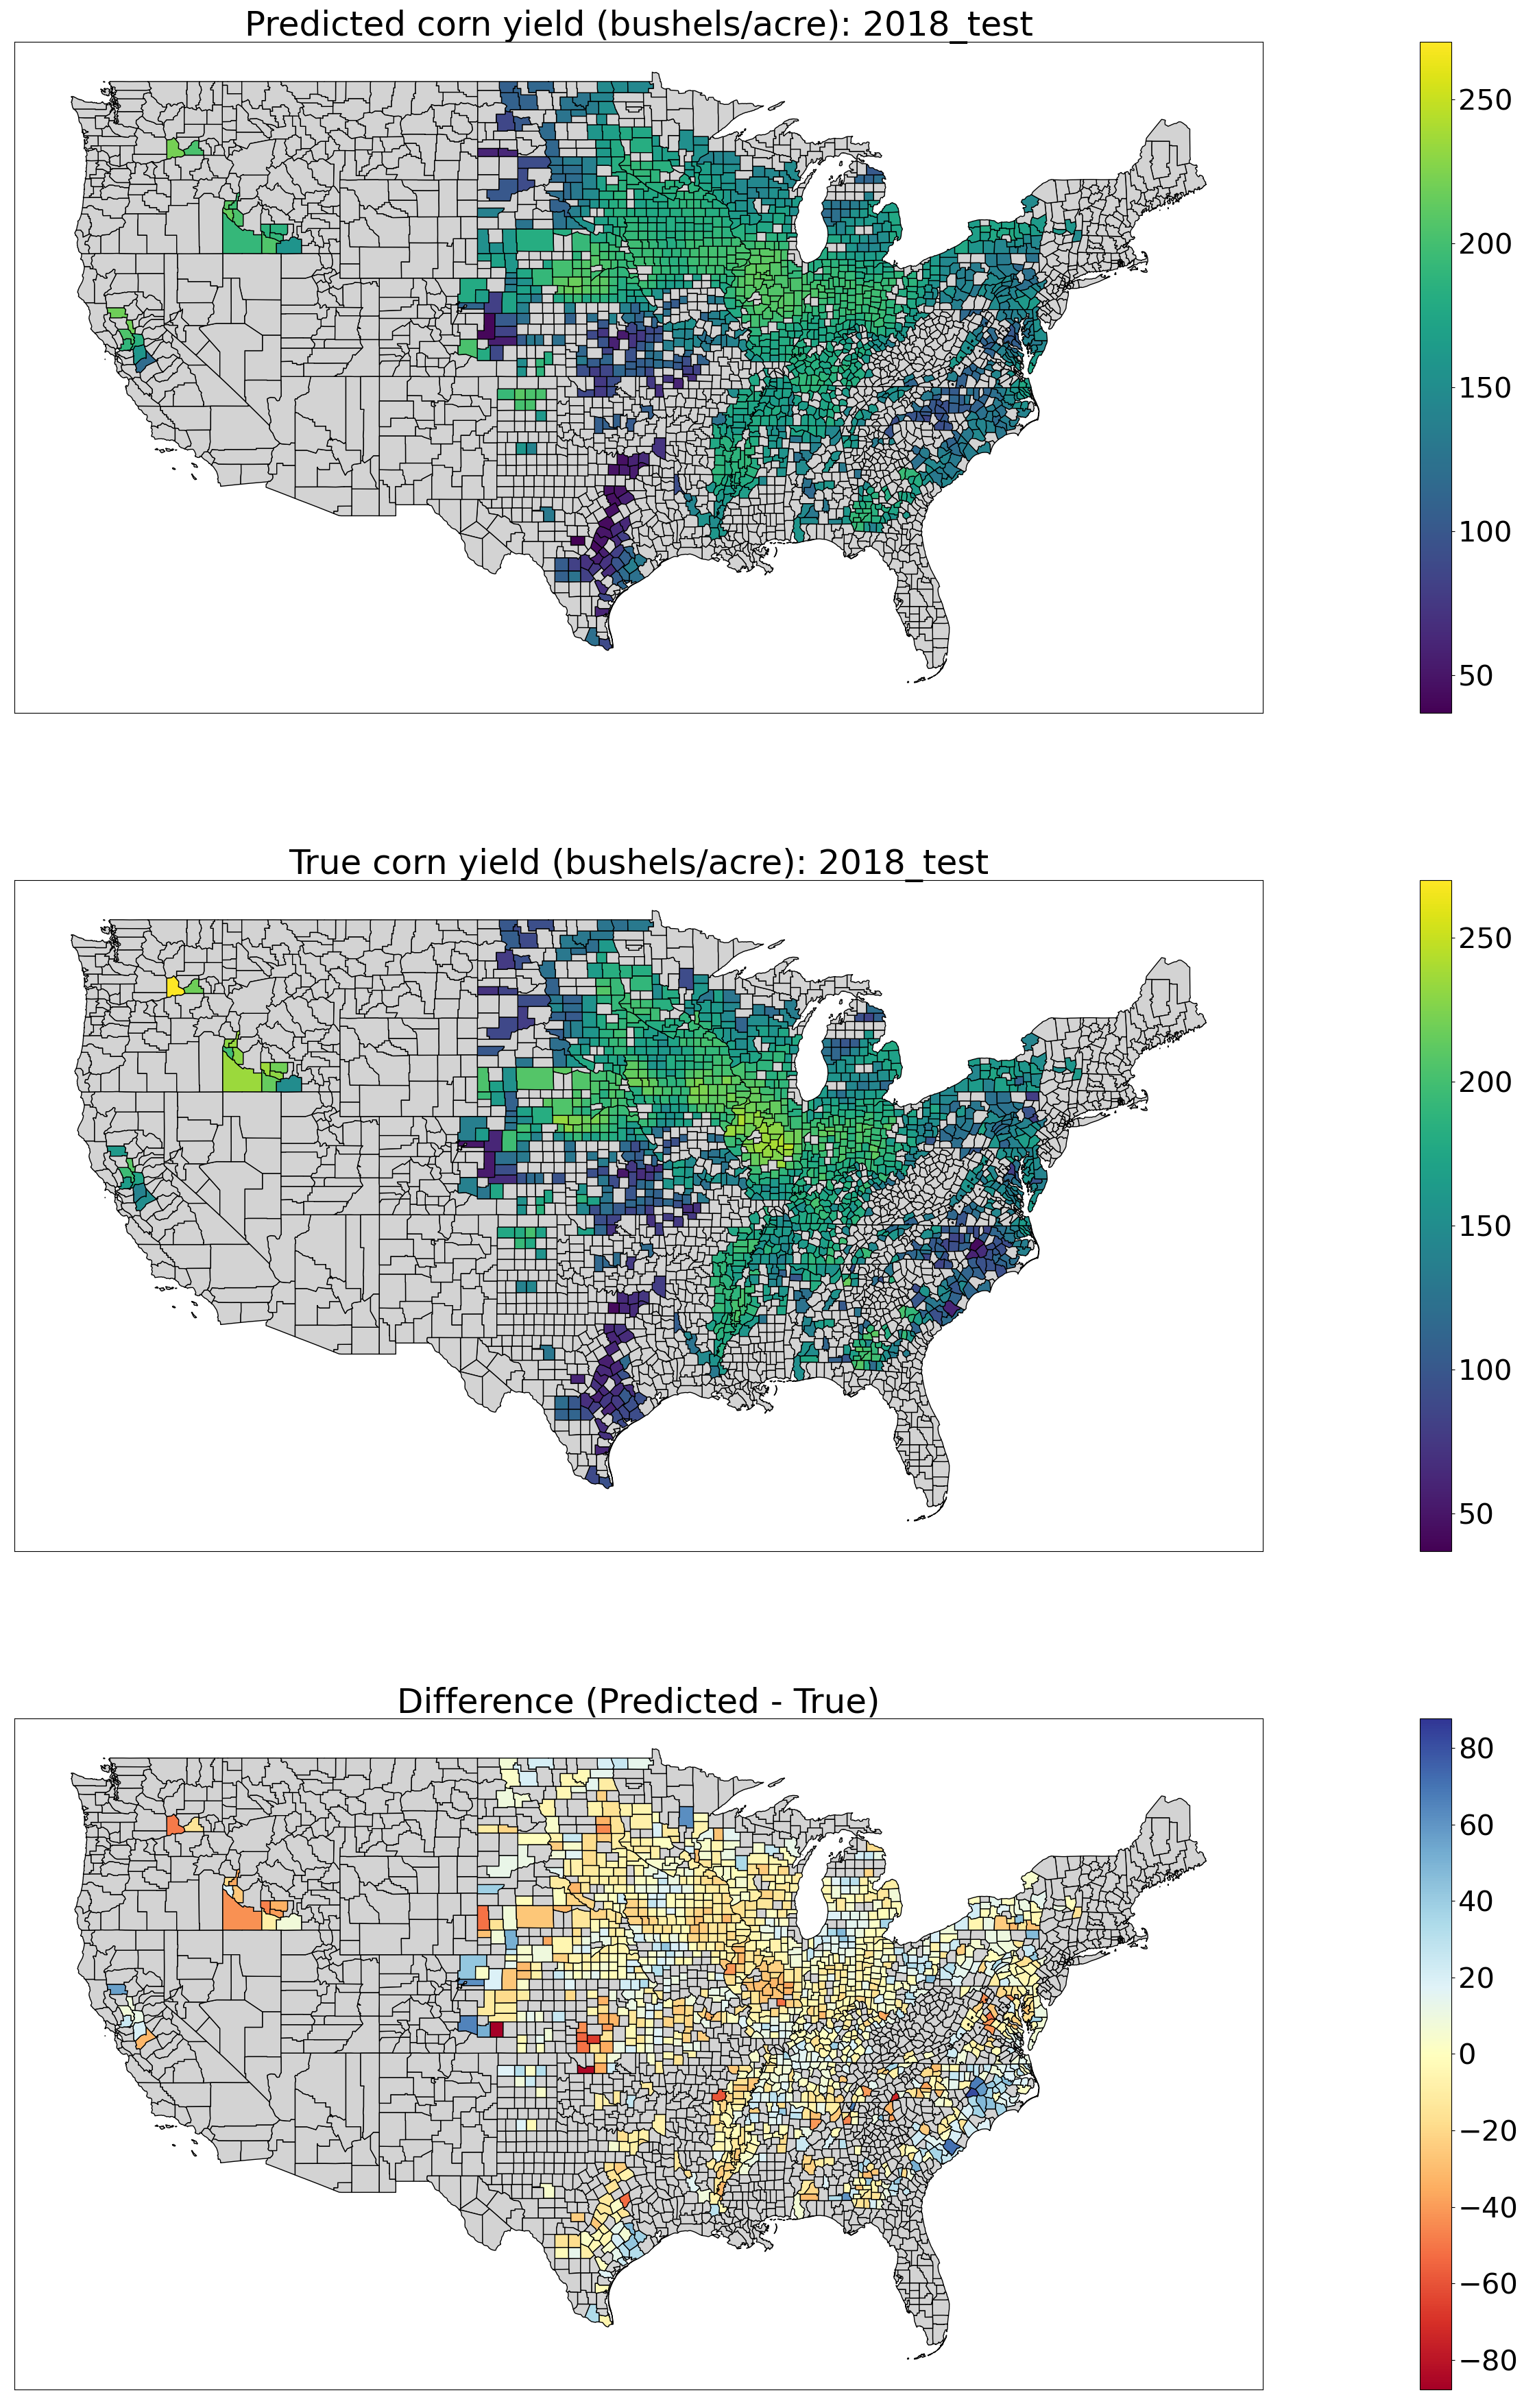
\includegraphics[width=0.95\columnwidth]{figs/true_vs_predicted_map_corn_2018_test.png}
\caption{Maps of predicted (top) and true (middle) corn yields in 2018, along with the difference (bottom). For the Difference plot, yellow means an accurate prediction, blue means the model predicted too high, and red means the model predicted too low. Gray means no data.}
\label{map}
\end{figure}

We evaluate the model on four test datasets: 2018 corn, 2018 soybean, 2019 corn, and 2019 soybean. These datasets span a wide geographic area, as well as differing growing conditions (2019 was a bad year due to the wet spring in the Midwest, which caused planting to be delayed). The results on these datasets are shown in Table \ref{results}. For the methods that only use 1 year when making predictions, our GNN model clearly outperforms comparable baselines across all datasets and metrics (except for 2018 soybean Corr, where it is slightly worse than GRU). For the methods that use a history of 5 years, our GNN-RNN outperforms competing baselines in almost all cases (except for 2018 soybean Corr, where it is slightly worse than CNN-RNN). For example, in 2019, our corn yield prediction on $R^2$ score is 16\% better than the prediction of a state-of-the-art work \cite{khaki2020cnn}. On average, we achieve a relative $R^2$ improvement of 10.44\% over the recent CNN-RNN model, 16.16\% over the 5-year LSTM, and a relative RMSE improvement of 9.6\% over the CNN-RNN model, 13.18\% over the 5-year LSTM.  These indicate the importance of exploiting geospatial context in making these predictions.




Figure \ref{scatter} shows an example scatterplot of true vs. predicted corn yields for the test year 2018. The GNN-RNN model is able to capture differences in yield between counties quite well. One minor issue is that the model is not able to capture the counties with very high yields very well; the model almost never predicts a yield higher than 220, but there are actually several counties with a true yield higher than this. This may stem from the fact that such high yields were almost never seen before in the training years. % (recall that yields tend to increase over the years). so the model is not trained to predict such high values.

We can also see these trends in the map (Figure \ref{map}). While the GNN-RNN model captures large-scale trends in crop yield very well, it sometimes outputs overly smooth predictions within a region, and under-predicts the area of high true yield in the Midwest. Improving the GNN's ability to detect fine-scale variations without smoothing them out is an important area for future work. 

We can see that crop yield prediction on a large scale is rather challenging, due to the complexity of the prediction task and the data involved. Each data point (one county/one year) has over 6,000 features, and standard models can easily overfit to noise in the data and fail to generalize. In order for the prediction task to be tractable, a model needs to take advantage of the various forms of structure in the data; temporal structure within a year (to capture weather patterns in different times of the year), temporal structure across years (to capture long-term trends such as technological improvements), and geospatial structure (to capture correlations between nearby county yields).  Our GNN-RNN model is the first model to take all of these aspects into account when making crop yield predictions, and achieves superior performance compared with the existing state-of-the-art. 

\subsection{Early Prediction}

In practice, crop yield predictions are most useful if they can be made well before harvest, as this gives time for markets to adapt, and humanitarian aid to be organized in cases of famine \cite{you2017deep}. To simulate this, at test time only, for each county we mask out all weather and land surface features from after June 1 (week 22) of the test year, and replace them with the average values for that county during the training years. Then we pass the masked features through a pre-trained model to obtain predictions. The results for several methods for 2018 corn are presented in Table \ref{early}. The graph-based models (GNN and GNN-RNN) clearly outperform competing baselines in this scenario, again illustrating the importance of utilizing geospatial context.



% \subsection{XXX}
% \junwen{qualitative results such as plots, and maybe some extra experiments depending on the space. otherwise, we put them to the supp}

\section{Conclusion}

In this paper, we propose a novel GNN-RNN framework to innovatively incorporate both geospatial and temporal knowledge into crop yield prediction, through graph-based deep learning methods. To our knowledge, our paper is the first to take advantage of the spatial structure in the data when making crop yield predictions, as opposed to previous approaches which assume that neighboring counties are independent samples. We conduct extensive experiments on large-scale datasets covering 41 US states and 39 years, and show that our approach substantially outperforms many existing state-of-the-art machine learning methods across multiple datasets. Thus, we demonstrate that incorporating knowledge about a county's geospatial neighborhood and recent  history can significantly enhance the prediction accuracy of deep learning methods for crop yield prediction. 

%, and demonstrate its superiority to existing models. large-scale crop yield dataset \textit{USCrop}, covering 48 states and 39 years. On \textit{USCrop}, we broadly compare the popular AI methods in crop yield prediction and provide solid baselines on three well-known metrics. Furthermore, we propose a novel GNN-RNN framework to innovatively incorporate both geospatial and temporal knowledge into prediction, through graph-based deep learning methods, and demonstrate its superiority to existing models. As far as we know, \textit{USCrop} is so far the most comprehensive crop yield dataset both spatially and temporally for machine learning. We will keep maintaining the dataset by including more features such as satellite images and progress data, and updating the dataset every year. We hope \textit{USCrop} can become a solid benchmark for crop yield study and an inspiration for novel machine learning techniques in spatiotemporal data modeling. We will also explore 
% more effective ways to better understand the influence of climatic variations. 

% In this paper, we present a large-scale crop yield dataset \textit{USCrop}, covering 48 states and 39 years. On \textit{USCrop}, we broadly compare the popular AI methods in crop yield prediction and provide solid baselines on three well-known metrics. Furthermore, we propose a novel GNN-RNN framework to innovatively incorporate both geospatial and temporal knowledge into prediction, through graph-based deep learning methods, and demonstrate its superiority to existing models. As far as we know, \textit{USCrop} is so far the most comprehensive crop yield dataset both spatially and temporally for machine learning. We will keep maintaining the dataset by including more features such as satellite images and progress data, and updating the dataset every year. We hope \textit{USCrop} can become a solid benchmark for crop yield study and an inspiration for novel machine learning techniques in spatiotemporal data modeling. We will also explore 
% more effective ways to better understand the influence of climatic variations. 

\section{Acknowledgements}

This research was supported by USDA Cooperative Agreement 58-6000-9-0041 and USDA NIFA Hatch Project 1017421. We would like to thank Rich Bernstein for constructive suggestions and Samuel Porter for help in processing the gSSURGO dataset.

%\clearpage
\bibliography{ref}

\clearpage
\appendix

\section{Supplemental Material}

\subsection{List of Features}

We provide a list of all of the input features used in the model, grouped by source. Note that all features are spatially aggregated to the county level, using a weighted average (where each grid cell is weighted by the fraction of the cell that lies inside the county, multiplied by the percentage of the grid cell that is cropland/pasture/grassland). An example of this aggregation process is depicted in Figure \ref{aggregating_to_county}. Temporally, all time-dependent features are also aggregated to weekly frequency.

\begin{figure}[h]
\centering
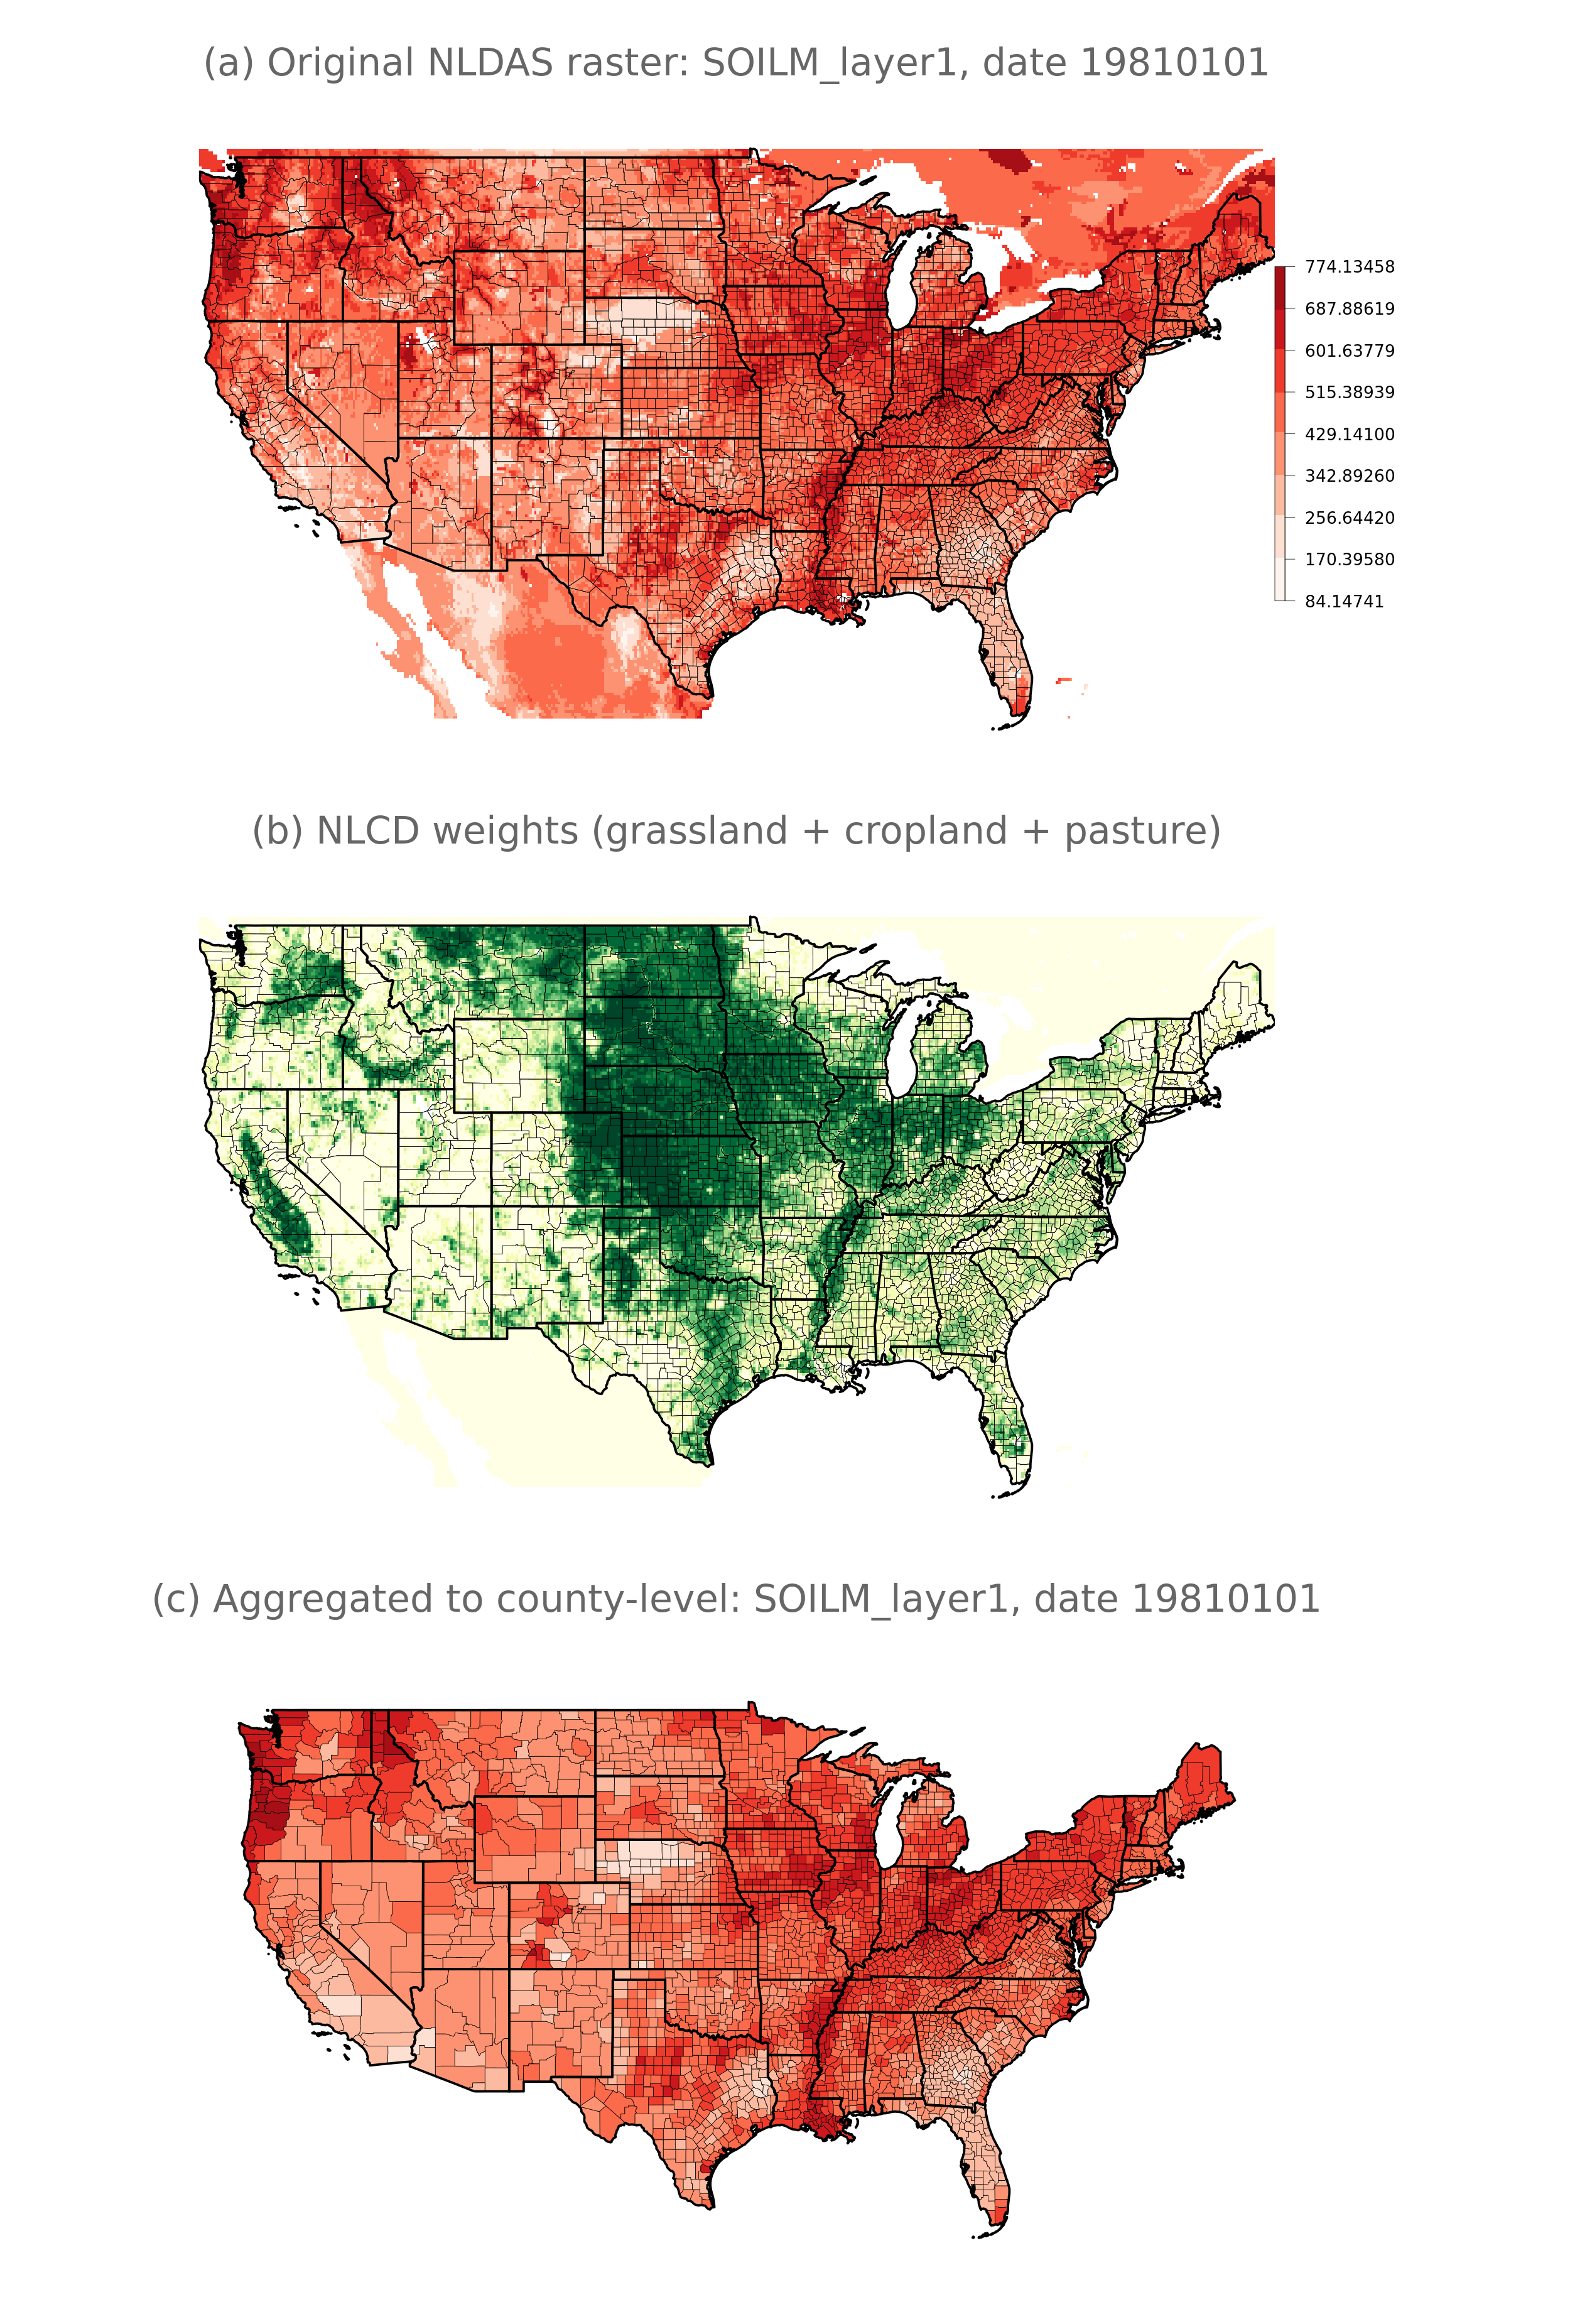
\includegraphics[width=0.9\columnwidth]{figs/nldas_SOILM_layer1_19810101_raster_and_weights.png}
\caption{Example of aggregating features to county level. \\
\textbf{(a)} raw raster of soil moisture from NLDAS. \\
\textbf{(b)} Percentage cropland/grassland/pasture (used to compute grid cell weights).\\
\textbf{(c)} the county-level values we generated.}
\label{aggregating_to_county}
\end{figure}


\textbf{Weather features} ($\mathbf{x}_{c,t}^w$) come from the PRISM dataset \cite{daly2013prism}, with an original spatial resolution of 4 km and a temporal resolution of daily:

\begin{enumerate}
    \item Precipitation
    \item Mean dewpoint temperature
    \item Daily max temperature
    \item Daily mean temperature
    \item Daily minimum temperature
    \item Max vapor pressure deficit
    \item Min vapor pressure deficit
\end{enumerate}

\textbf{Land surface features} ($\mathbf{x}_{c,t}^l$) come from the NLDAS land surface model \cite{xia2012continental}, with an original spatial resolution of 0.125 degrees (14 km) and a temporal resolution of hourly:

\begin{enumerate}
    \item Precipitation hourly total (kg/$m^2$)
    \item Moisture availability (\%), 0-200 cm
    \item Moisture availability (\%), 0-100 cm
    \item Soil moisture content (kg/$m^2$), 0-200cm
    \item Soil moisture content (kg/$m^2$), 0-100cm
    \item Soil moisture content (kg/$m^2$), 0-10cm
    \item Soil moisture content (kg/$m^2$), 10-40cm
    \item Soil moisture content (kg/$m^2$), 40-100cm
    \item Soil moisture content (kg/$m^2$), 100-200cm
    \item 2-m above ground specific humidity (kg/kg)
    \item 2-m above ground temperature (K)
    \item Soil temperature (K), 0-10 cm
    \item Soil temperature (K), 10-40 cm
    \item Soil temperature (K), 40-100 cm
    \item Soil temperature (K), 100-200 cm
    \item Wind speed (m/s), hourly max
\end{enumerate}

(Note that the cm ranges represent depths in the soil.)\\

 \textbf{Soil quality features} ($\mathbf{x}_{c}^s$) come from the Gridded Soil Survey Geographic Database (gSSURGO) \cite{soil2019gridded}. The dataset has a 30-m spatial resolution for the continental U.S. These variables do not change over time. However, they vary with depths, which are measured at 6 soil depth layers (0-5cm, 5-15cm, 15-30cm, 30-60cm, 60-100cm, 100-200cm). Because soil quality at a given point can vary substantially within a county, accounting for the location of agricultural activity can be critical when constructing appropriate county-level soil variables. Thus, the ``weighted-average'' technique is especially important here. We aggregate the fine-scale soil data to the county level based on the percentage of each NLCD Land Cover grid cell that was covered by agricultural land (grassland, pasture, cropland) in 2011.
 
\begin{enumerate}
    \item Available water capacity of the dominant soil component
    \item Bulk density
    \item Electrical conductivity of the dominant soil component
    \item Organic matter
    \item Average \% silt
    \item Average \% clay
    \item Average \% sand
    \item \% area covered by Clay soil type
    \item \% area covered by Silty Clay soil type
    \item \% area covered by Sandy Clay soil type
    \item \% area covered by Clay Loam soil type
    \item \% area covered by Silty Clay Loam soil type
    \item \% area covered by Sandy Clay Loam soil type
    \item \% area covered by Loam soil type
    \item \% area covered by Silt Loam soil type
    \item \% area covered by Sandy Loam soil type
    \item \% area covered by Silt Loam soil type
    \item \% area covered by Loamy Sand soil type
    \item \% area covered by Sand soil type
    \item pH, which is influenced by chemical reactions between water and the dominant soil component
\end{enumerate}
Note that features 8-19 were not present in the original gSSURGO dataset. Rather, for each pixel, we used the raw silt, clay, and sand percentages to compute the ``soil texture type'' of that pixel, based on the National Resources Conservation Service Soil Survey's classification scheme \cite{soiltexture}. This classification scheme is depicted in Figure \ref{soil_triangle}. After classifying each pixel's soil texture type, we compute the fraction of each county that is occupied by each soil texture type.

\begin{figure}[bt]
\centering
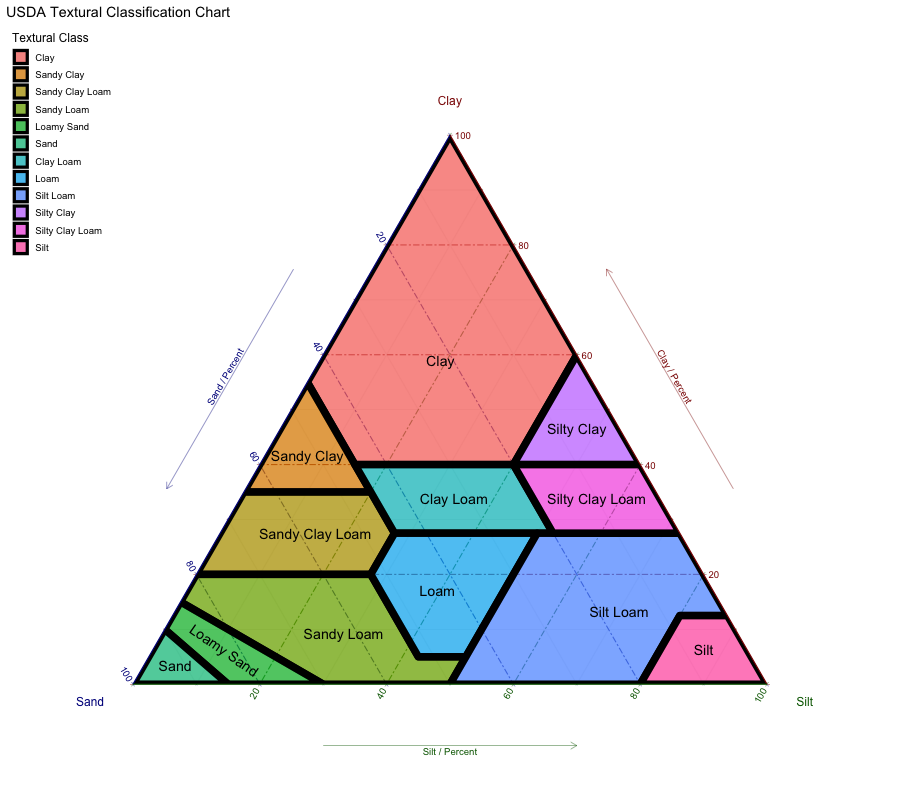
\includegraphics[width=0.95\columnwidth]{figs/soil_triangle.png}
\caption{NRCS Soil Texture classification \cite{soiltexture}. The three sides of the triangle represent percentage sand, clay, and silt, and the colored regions are the soil texture types.}
\label{soil_triangle}
\end{figure}

\textbf{Extra features} ($\mathbf{x}_{c}^e$) also come from the gSSURGO dataset \cite{soil2019gridded}, but are not depth-dependent. They are listed below:

\begin{enumerate}
    \item National commodity crop productivity index
    \item Depth to any soil restrictive layer
    \item NCCPI crop productivity index for small grains, weighted average
    \item NCCPI crop productivity index for corn
    \item NCCPI crop productivity index for cotton
    \item NCCPI crop productivity index for soybean
\end{enumerate}
% \begin{table}[]
% \centering
% % \fontsize{9}{10}\selectfont
% \begin{tabular}{|l|c|c|c|} \hline
% \textbf{Data source} & \textbf{Original temporal resolution} & \textbf{Original spatial resolution} & \textbf{Features} \\ \hline
% PRISM & & & \\
% \end{tabular}
% \caption{2019 soybean results}
% \label{2019_soybean}
% \end{table}




\subsection{Hyperparameter Details}

For all methods, we use the Adam optimizer \cite{kingma2014adam}. For the CNN-RNN, GNN, and GNN-RNN methods, we tried many hyperparameter configurations, most intensively on the 2018 corn dataset. We tried learning rates from \{1e-5, 2e-5, 5e-5, 1e-4, 2e-4, 5e-4, 1e-3\}, used a weight decay of 1e-5 or 1e-4, and a batch size of 32, 64, or 128. We tried using a mild cosine decay (with $\eta_{min} \in $ \{1e-5, 1e-6\}, $T_0 \in \{34, 100, 200\}$), or step decay (every 25 epochs, $\gamma \in \{0.5, 0.8\}$) for the learning rate scheduler. We trained the model for 100 to 200 epochs (until the validation loss clearly stopped improving). We chose the epoch and hyperparameter setting that produced the lowest RMSE on the validation year (the year before the test year).

For the GNN and GNN-RNN models, we used the implementation of GraphSAGE from the dgl library; we used a 2-layer GNN, with edge dropout of 0.1. We used stochastic mini-batch training to train the model, where each layer samples 10 neighbors to receive messages from. We tried different aggregation functions, such as ``mean'' and ``pooling.''



We ran the GNN-RNN model 3 times with random seeds \{0, 1, 2\} to evaluate the variance in the results. For the baseline models, we used seed 0. The final hyperparameter configurations are listed in the below tables.

% main.py --dataset corn_weekly --data_dir /mnt/beegfs/bulk/mirror/jyf6/datasets/crop_forecast/data/combined_dataset_weekly.npz -adj ../map/us_adj.pkl --crop_id_to_fid ../map/soybean_fid_dict.pkl --mode train --length 5 -bs 128 --max_epoch 100 --test_year 2019 --model cnn_rnn -lr 1e-4 --eta_min 1e-5 --check_freq 80 --T0 50 -sche step --crop_type corn --num_weather_vars 23 --num_management_vars 96 --num_soil_vars 20 --num_extra_vars 6 --soil_depths 6
\begin{table}[H]
\centering
% \fontsize{9}{10}\selectfont
\begin{tabular}{|l|l|} \hline
\textbf{Hyperparameter} & \textbf{Value} \\ \hline
Batch size & 128 \\ \hline
Learning rate & 1e-4\\ \hline
LR scheduling & Step (25 epochs, $\gamma$ = 0.5)  \\ \hline
Number of epochs & 100 \\ \hline
Weight decay & 1e-5 \\ \hline
\end{tabular}
\caption{CNN-RNN hyperparameters: corn}
\label{hyperparams_cnn-rnn_corn}
\end{table}

\begin{table}[H]
\centering
% \fontsize{9}{10}\selectfont
\begin{tabular}{|l|l|} \hline
\textbf{Hyperparameter} & \textbf{Value} \\ \hline
Batch size & 128 \\ \hline
Learning rate & 5e-4 \\ \hline
LR scheduling & Step (25 epochs, $\gamma$ = 0.5)  \\ \hline
Number of epochs & 100 \\ \hline
Weight decay & 1e-5 \\ \hline
\end{tabular}
\caption{CNN-RNN hyperparameters: soybeans}
\label{hyperparams_cnn-rnn_soybean}
\end{table}

% python main.py --dataset corn_weekly --data_dir /mnt/beegfs/bulk/mirror/jyf6/datasets/crop_forecast/data/combined_dataset_weekly.npz  \
%     -adj ../map/us_adj.pkl --crop_id_to_fid ../map/soybean_fid_dict.pkl \
%     --mode train --length 5 -bs $1 --max_epoch 70 --test_year 2018 -lr $2 \
%     --eta_min 1e-5 --check_freq 80 --T0 200 -sche $3 --dropout 0.1 --z_dim 64 \
%     --crop_type corn --num_weather_vars 23 --num_management_vars 96 --num_soil_vars 20 --num_extra_vars 6 --soil_depths 6 --no_management --aggregator_type $4 \
%     --note $5
%./run_train.sh 32 1e-4 cosine pool day_0
\begin{table}[H]
\centering
% \fontsize{9}{10}\selectfont
\begin{tabular}{|l|l|} \hline
\textbf{Hyperparameter} & \textbf{Value} \\ \hline
Batch size & 32 \\ \hline
Learning rate & 1e-4 \\ \hline
LR scheduling & Cosine ($T_0 = 200, \eta_{min} = 10^{-5}$)  \\ \hline
Number of epochs & 100 \\ \hline
Weight decay & 1e-5 \\ \hline
GNN edge dropout & 0.1 \\ \hline
GNN aggregator & pool \\ \hline
\end{tabular}
\caption{GNN hyperparameters: corn, 2018}
\label{hyperparams_gnn_corn_2018}
\end{table}

% % "python main.py --dataset corn_weekly --data_dir /mnt/beegfs/bulk/mirror/jyf6/datasets/crop_forecast/data/combined_dataset_weekly.npz  \
%     -adj ../map/us_adj.pkl --crop_id_to_fid ../map/soybean_fid_dict.pkl \
%     --mode train --length 5 -bs $1 --max_epoch 200 --test_year 2019 -lr $2 \
%     --eta_min 1e-5 --check_freq 80 --T0 100 -sche $3 --dropout 0. --z_dim 64 \
%     --crop_type corn --num_weather_vars 23 --num_management_vars 96 --num_soil_vars 20 --num_extra_vars 6 --soil_depths 6 --no_management \
%     --note $4
% # ./run_train.sh 64 5e-5 cosine day_0"
\begin{table}[H]
\centering
% \fontsize{9}{10}\selectfont
\begin{tabular}{|l|l|} \hline
\textbf{Hyperparameter} & \textbf{Value} \\ \hline
Batch size & 64 \\ \hline
Learning rate & 5e-5 \\ \hline
LR scheduling & Cosine ($T_0 = 100, \eta_{min} = 10^{-5}$)  \\ \hline
Number of epochs & 200 \\ \hline
Weight decay & 1e-5 \\ \hline
GNN edge dropout & 0 \\ \hline
GNN aggregator & mean \\ \hline
\end{tabular}
\caption{GNN hyperparameters: corn, 2019}
\label{hyperparams_gnn_corn_2019}
\end{table}


% model/soybeans_weekly/2018/gnn_bs-64_lr-0.0001_maxepoch-100_sche-step_T0-25_step-25_gamma-0.8_dropout-0.1_testyear-2018_aggregator-pool_encoder-cnn_trainweekstart-52_len-5_seed-1_no-management/model-58
% model/soybeans_weekly/2019/gnn_bs-64_lr-0.0001_maxepoch-100_sche-step_T0-25_step-25_gamma-0.8_dropout-0.1_testyear-2019_aggregator-pool_encoder-cnn_trainweekstart-52_len-5_seed-2_no-management/model-15
\begin{table}[H]
\centering
% \fontsize{9}{10}\selectfont
\begin{tabular}{|l|l|} \hline
\textbf{Hyperparameter} & \textbf{Value} \\ \hline
Batch size & 64 \\ \hline
Learning rate & 1e-4 \\ \hline
LR scheduling & Step (25 epochs, $\gamma = 0.8$)  \\ \hline
Number of epochs & 100 \\ \hline
Weight decay & 1e-5 \\ \hline
GNN edge dropout & 0.1 \\ \hline
GNN aggregator & pool \\ \hline
\end{tabular}
\caption{GNN hyperparameters: soybeans, 2018 and 2019}
\label{hyperparams_gnn_soybeans_2018}
\end{table}

% model/corn_weekly_no_Y_input_shuffle/2018/gnn-rnn_bs-32_lr-5e-05_maxepoch-100_sche-cosine_T0-100_etamin-1e-06_step-25_gamma-1.0_dropout-0.1_sleep-100_testyear-2018_aggregator-pool_encoder-cnn_trainweekstart-52_len-5_weightdecay-1e-05_seed-2_no-management/model-72
\begin{table}[H]
\centering
% \fontsize{9}{10}\selectfont
\begin{tabular}{|l|l|} \hline
\textbf{Hyperparameter} & \textbf{Value} \\ \hline
Batch size & 32 \\ \hline
Learning rate & 5e-5 \\ \hline
LR scheduling & Cosine ($T_0 = 100, \eta_{min} = 10^{-6}$)  \\ \hline
Number of epochs & 100 \\ \hline
Weight decay & 1e-5 \\ \hline
GNN edge dropout & 0.1 \\ \hline
GNN aggregator & pool \\ \hline
\end{tabular}
\caption{GNN-RNN hyperparameters: corn, 2018}
\label{hyperparams_gnn_corn_2018}
\end{table}

%model/corn_weekly_no_Y_input_shuffle/2019/gnn-rnn_bs-32_lr-5e-05_maxepoch-100_sche-cosine_T0-200_etamin-1e-06_step-25_gamma-1.0_dropout-0.1_sleep-100_testyear-2019_aggregator-pool_encoder-cnn_trainweekstart-52_len-5_weightdecay-1e-05_seed-2_no-management/model-88
\begin{table}[H]
\centering
% \fontsize{9}{10}\selectfont
\begin{tabular}{|l|l|} \hline
\textbf{Hyperparameter} & \textbf{Value} \\ \hline
Batch size & 32 \\ \hline
Learning rate & 5e-5 \\ \hline
LR scheduling & Cosine ($T_0 = 200, \eta_{min} = 10^{-6}$)  \\ \hline
Number of epochs & 100 \\ \hline
Weight decay & 1e-5 \\ \hline
GNN edge dropout & 0.1 \\ \hline
GNN aggregator & pool \\ \hline
\end{tabular}
\caption{GNN-RNN hyperparameters: corn, 2019}
\label{hyperparams_gnn_corn_2019}
\end{table}


%model/soybeans_weekly_no_Y_input_shuffle/2018/gnn-rnn_bs-32_lr-0.0001_maxepoch-100_sche-cosine_T0-100_etamin-1e-06_step-25_gamma-1.0_dropout-0.1_sleep-100_testyear-2018_aggregator-pool_encoder-cnn_trainweekstart-52_len-5_weightdecay-0.0001_seed-2_no-management/model-42
%
\begin{table}[H]
\centering
% \fontsize{9}{10}\selectfont
\begin{tabular}{|l|l|} \hline
\textbf{Hyperparameter} & \textbf{Value} \\ \hline
Batch size & 32 \\ \hline
Learning rate & 1e-4 \\ \hline
LR scheduling & Cosine ($T_0 = 100, \eta_{min} = 10^{-6}$)  \\ \hline
Number of epochs & 100 \\ \hline
Weight decay & 1e-4 \\ \hline
GNN edge dropout & 0.1 \\ \hline
GNN aggregator & pool \\ \hline
\end{tabular}
\caption{GNN-RNN hyperparameters: soybeans, 2018}
\label{hyperparams_gnn_soybeans, 2018}
\end{table}

%model/soybeans_weekly_no_Y_input_shuffle/2019/gnn-rnn_bs-32_lr-5e-05_maxepoch-100_sche-cosine_T0-100_etamin-1e-06_step-25_gamma-1.0_dropout-0.1_sleep-100_testyear-2019_aggregator-pool_encoder-cnn_trainweekstart-52_len-5_weightdecay-1e-05_seed-0_no-management/model-18
\begin{table}[H]
\centering
% \fontsize{9}{10}\selectfont
\begin{tabular}{|l|l|} \hline
\textbf{Hyperparameter} & \textbf{Value} \\ \hline
Batch size & 32 \\ \hline
Learning rate & 5e-5 \\ \hline
LR scheduling & Cosine ($T_0 = 100, \eta_{min} = 10^{-6}$)  \\ \hline
Number of epochs & 100 \\ \hline
Weight decay & 1e-5 \\ \hline
GNN edge dropout & 0.1 \\ \hline
GNN aggregator & pool \\ \hline
\end{tabular}
\caption{GNN-RNN hyperparameters: soybeans, 2019}
\label{hyperparams_gnn_soybeans, 2019}
\end{table}


\subsection{Evaluation Metrics}

We evaluate our model across all counties in the test year with data. We use three standard regression metrics: RMSE, $R^2$, and Pearson correlation coefficient (Corr). 

The RMSE is the square root of the mean squared error between the prediction and the true value:

$$RMSE = \sqrt{\frac{\sum_c (y_c - \widehat{y_c})^2}{N}}$$

where $y_c$ is the true yield for county $c$, $\widehat{y_c}$ is the model's predicted yield for county $c$, and $N$ is the total number for counties in the test set with yield data. In this paper, we further divide RMSE by the standard deviation of the current crop's yield (across all years), in order to make the results for different crops comparable.

$R^2$ is a measure of how much the variation in the data can be explained by the model predictions. Formally,

$$R^2 = 1 - \frac{\sum_c (y_c - \widehat{y_c})^2}{\sum_c (y_c - \bar{y})^2}$$

where $\bar{y}$ is the average yield across the entire test dataset. The top of the fraction is the sum of the squared residuals (difference between true yield and model prediction). The bottom is the total sum of squares (of the difference between the true yield and the average yield across the test dataset), which is proportional to the overall variance of the test data. 

The Pearson correlation coefficient (Corr) measures the strength of the linear correlation between the true and predicted values. The correlation between two variables $x$ and $y$ is given as

$$r_{xy} = \frac{\sum_{i=1}^n (x_i - \bar{x}) (y_i - \bar{y})}{\sqrt{\sum_{i=1}^n (x_i - \bar{x})^2} \sqrt{\sum_{i=1}^n (y_i - \bar{y})^2}}$$

Again $\bar{x}$ and $\bar{y}$ are the means of $x$ and $y$ respectively. We let $x$ be the model prediction and $y$ be the true yield.










\subsection{Data and Code Availability}

We are planning to submit an expanded version of this paper to a journal, such as in the field of agricultural economics. After the journal article is published, we plan to make the entire aggregated dataset and codebase publicly available. All of the raw data used comes from publicly available sources. For now, we have submitted a data appendix with a small subset of the aggregated county-level data (only the states of Illinois and Iowa), and a code appendix containing our implementation of the GNN-RNN model. 

\begin{figure}[t]
\centering
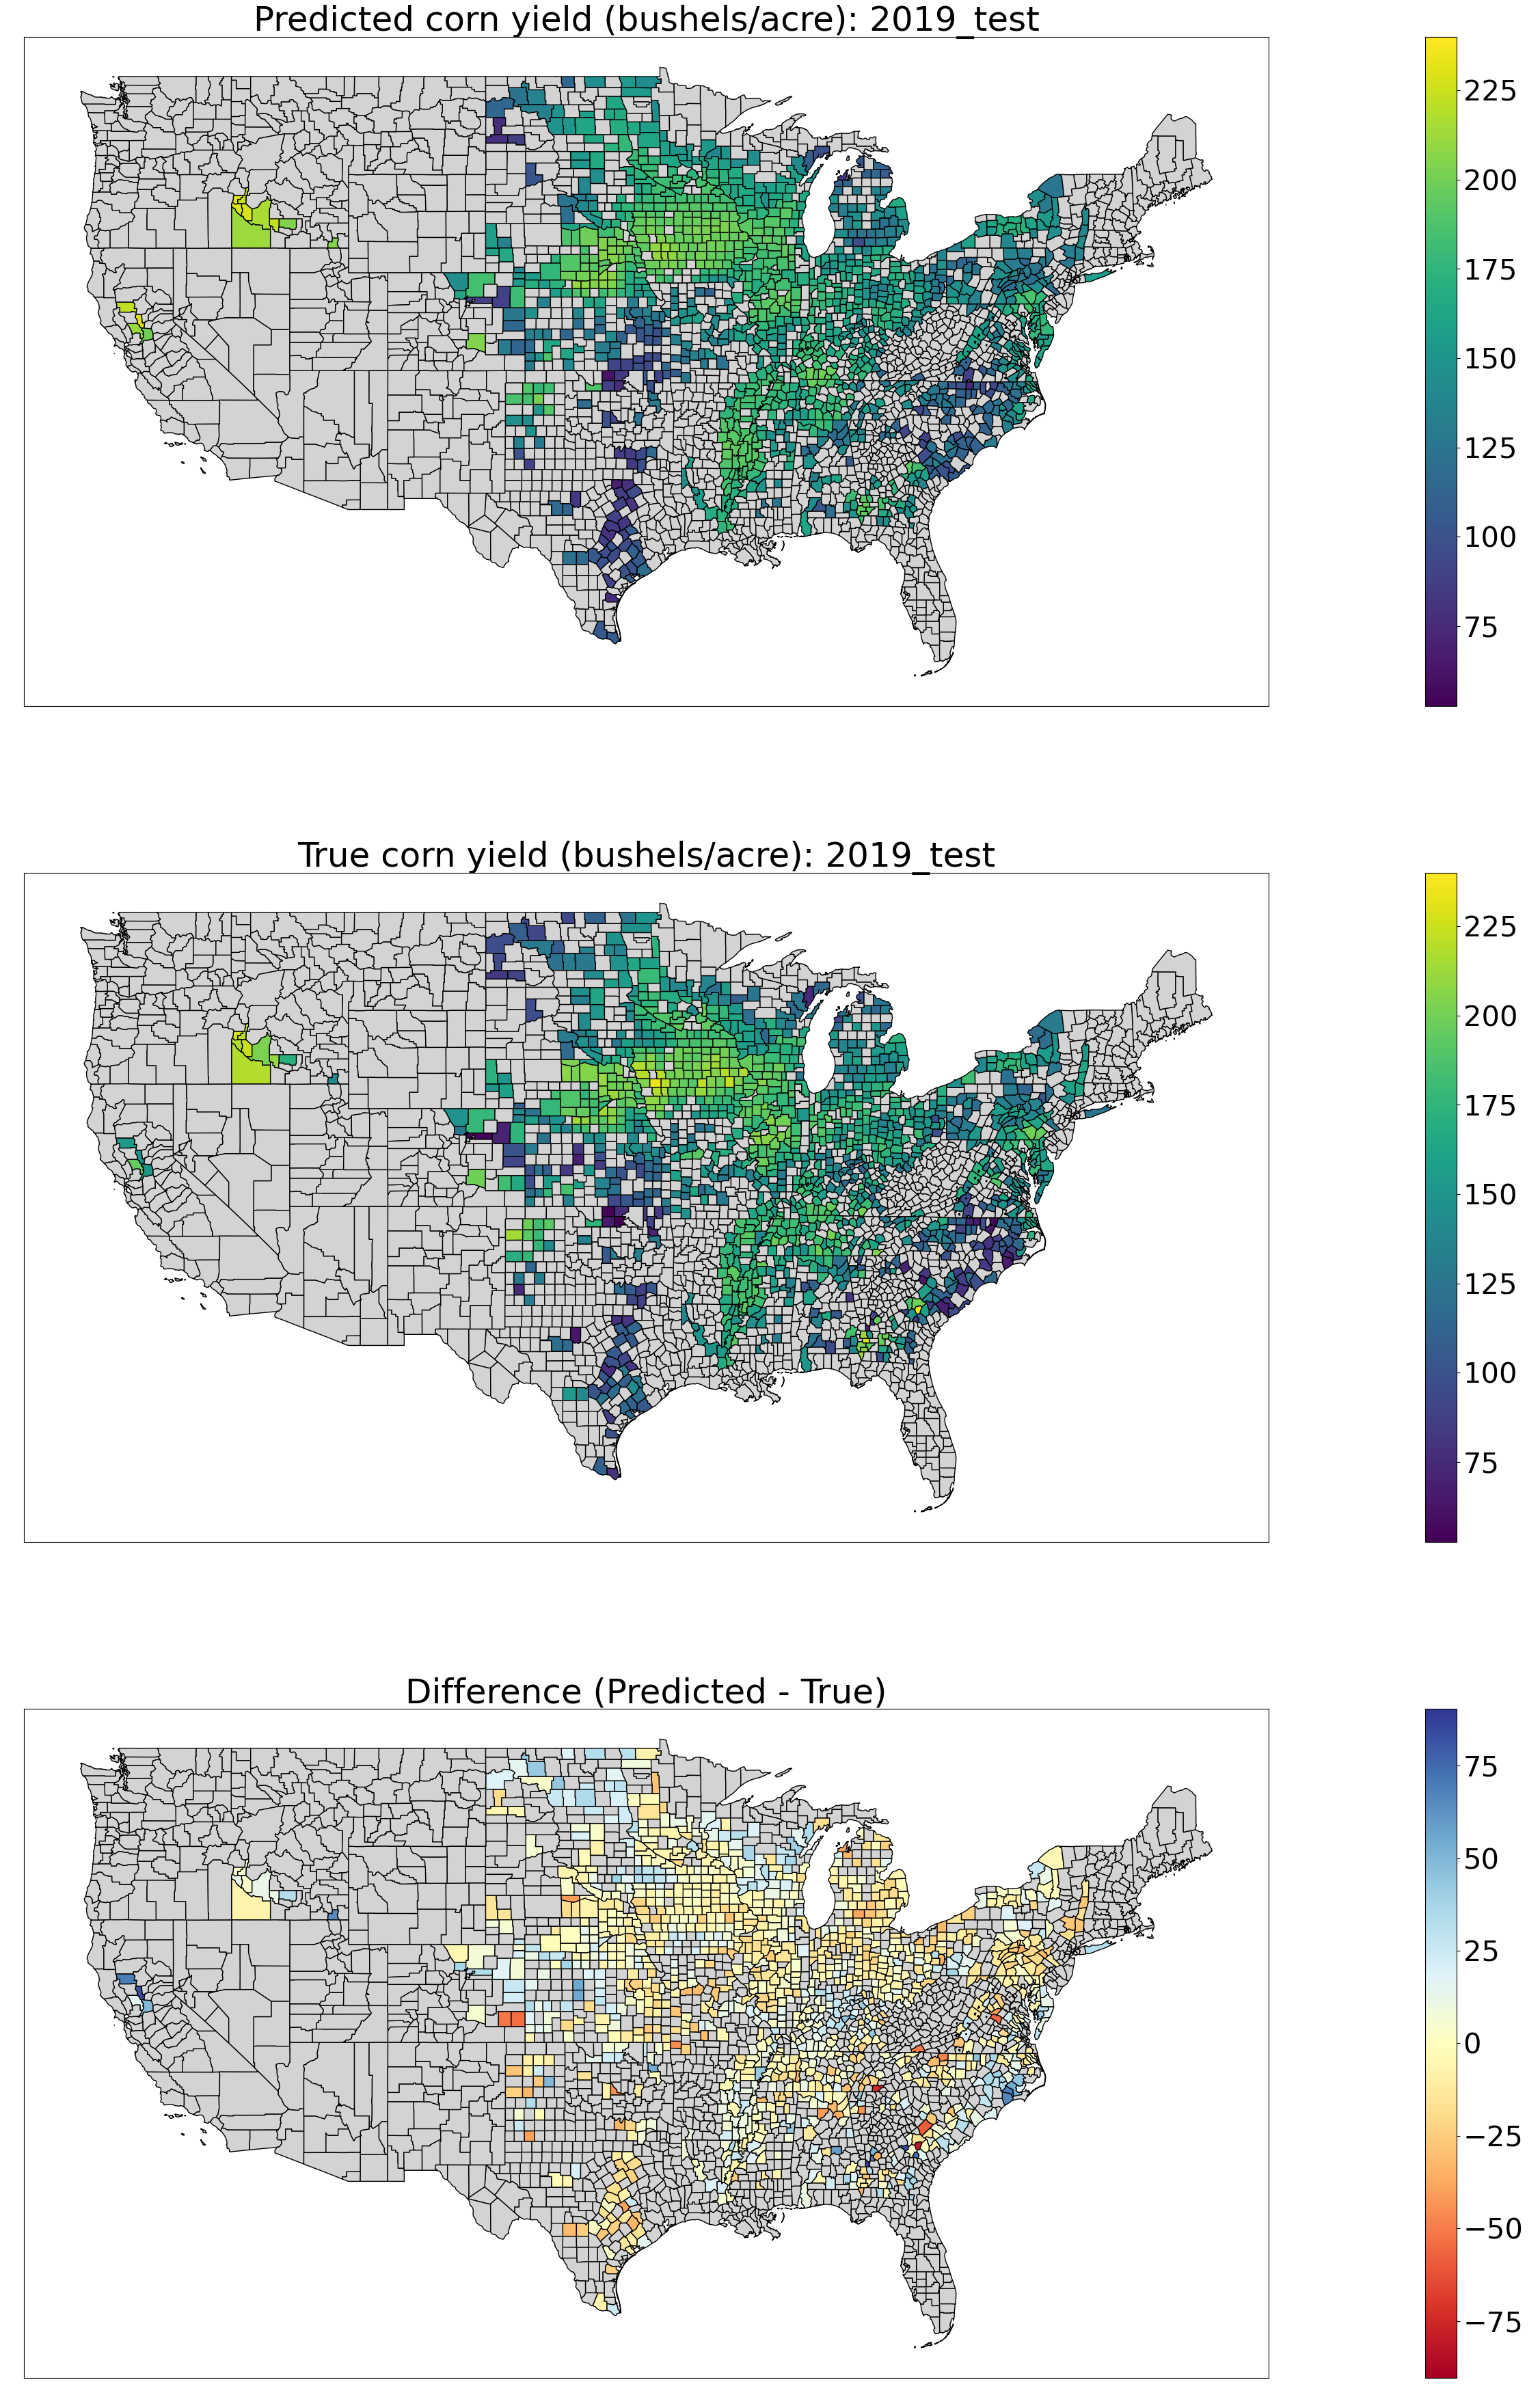
\includegraphics[width=0.95\columnwidth]{figs/true_vs_predicted_map_corn_2019_test.png}
\caption{2019 corn: Maps of predicted (top) and true (middle) yields, along with the difference (bottom).}
\label{fig:map_2019corn}
\vspace{-1em}
\end{figure}
\begin{figure}[H]
\centering
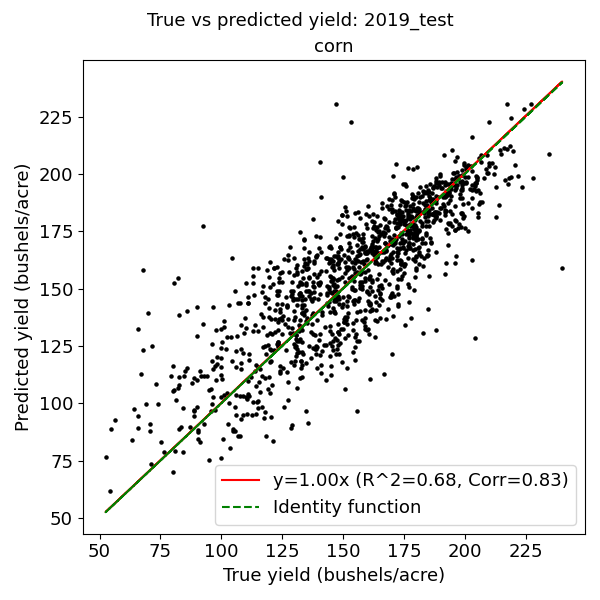
\includegraphics[width=0.8\columnwidth]{figs/true_vs_predicted_scatter_corn_2019_test.png}
\caption{2019 corn: Predicted vs. ground truth yields}
\label{fig:scatter_2019corn}
\end{figure}


\begin{figure}[H]
\centering
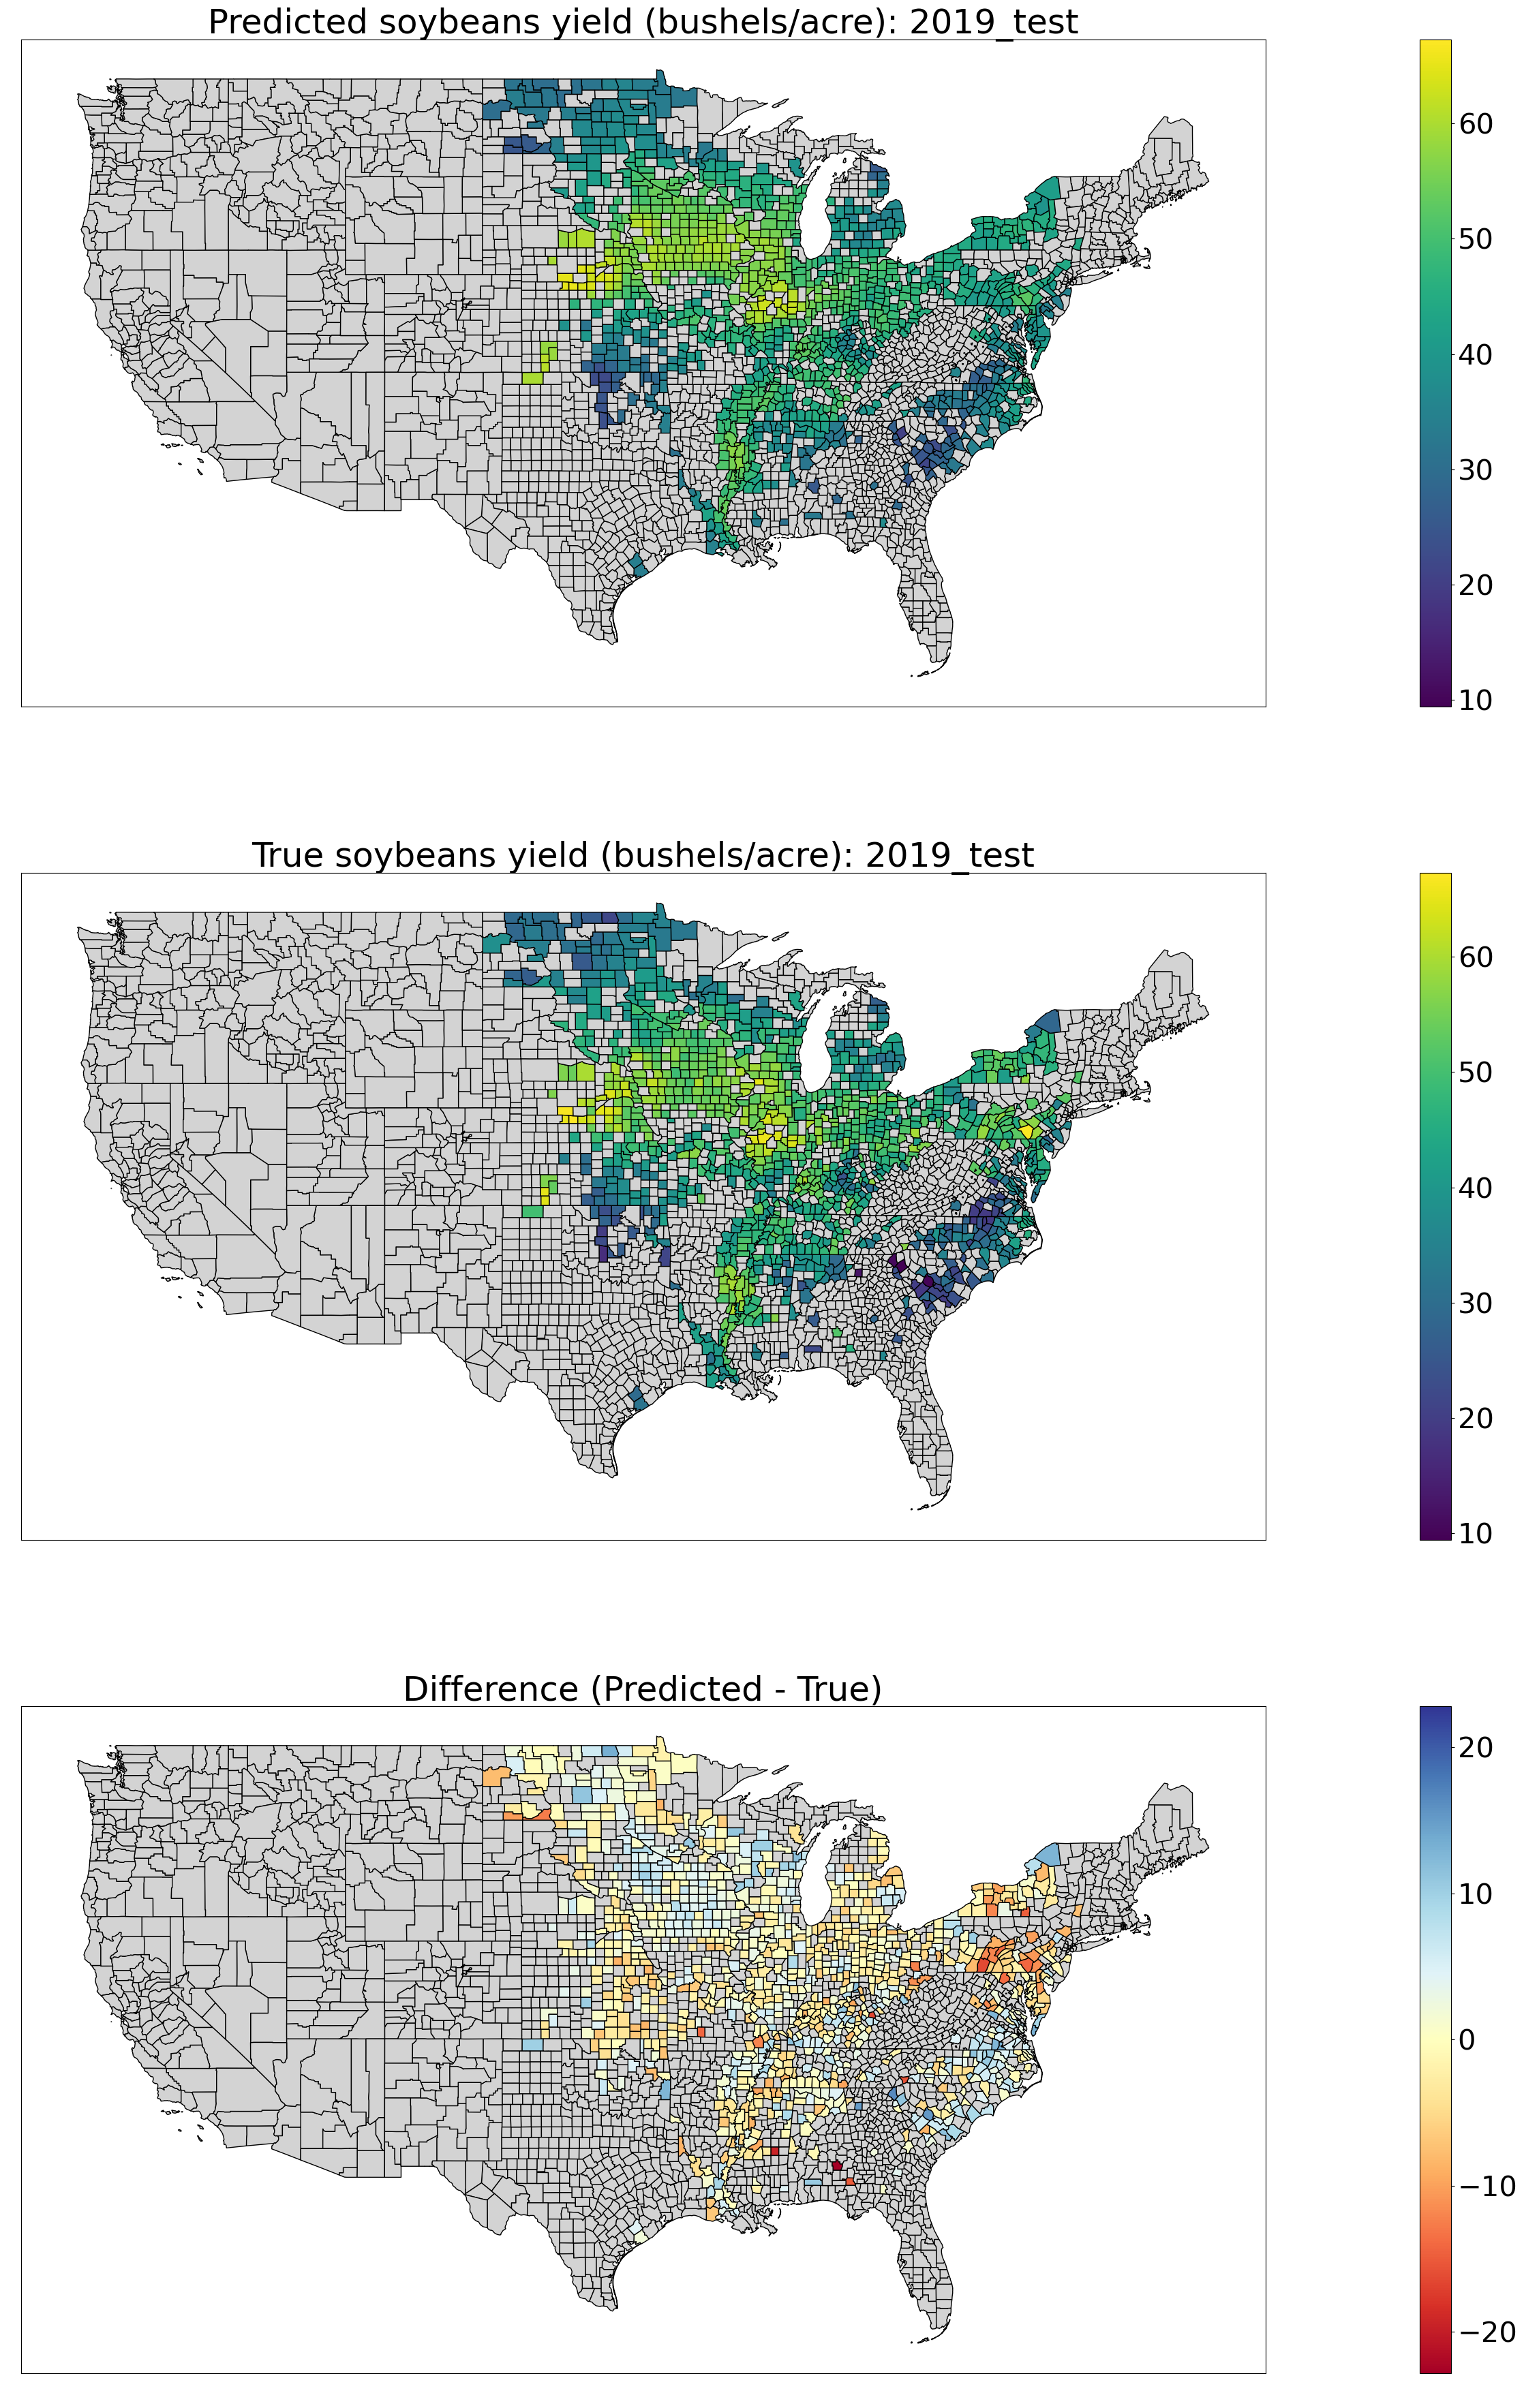
\includegraphics[width=0.95\columnwidth]{figs/true_vs_predicted_map_soybeans_2019_test.png}
\caption{2019 soybeans: Maps of predicted (top) and true (middle) yields, along with the difference (bottom).}
\label{fig:map_2019soy}
\end{figure}
\begin{figure}[H]
\centering
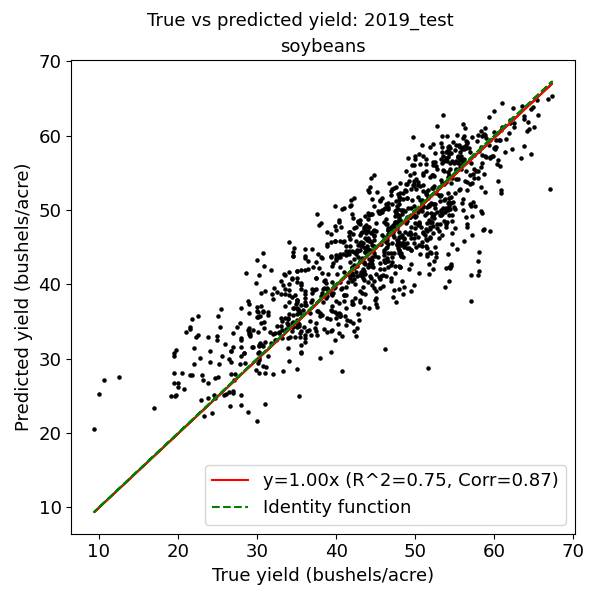
\includegraphics[width=0.8\columnwidth]{figs/true_vs_predicted_scatter_soybeans_2019_test.png}
\caption{2019 soybeans: Predicted vs. ground truth yields}
\label{fig:scatter_2019soy}
\end{figure}


\subsection{Computing Setup}

We ran our code on Python 3.7, using the following libraries: PyTorch 1.8, DGL 0.7.1, NumPy 1.18.5, SciPy 1.2.0. We trained on NVIDIA Tesla V100 GPU with 16GB memory, and used 12 CPU threads for GNN-RNN. The GNN-RNN model takes roughly 8 hours to train for 100 epochs on our full US dataset.



\subsection{Additional plots}

Here are maps and scatter plots showing example results for the GNN-RNN model on the other datasets.


\textbf{2019 corn:} Fig.~\ref{fig:map_2019corn} describes the difference between the ground-truth corn yields for counties in 2019, and our predictions. To demonstrate the similarity, we plot their difference in the bottom figure. As shown in the bottom sub-figure, almost all differences are all close to 0. Fig.~\ref{fig:scatter_2019corn} shows another plot of true-vs-predicted comparison. All the dots cling to the identity function, which means good prediction results.


\textbf{2019 soybeans:} Fig.~\ref{fig:map_2019soy} and Fig.~\ref{fig:scatter_2019soy} are similar true-vs-predicted plots for soybeans. The prediction results are also promising.




% \subsection{Early prediction results for soybean}

% Skip if not enough time


\end{document}
